% !TEX program = xelatex
\documentclass[UTF8,fontset=fandol,a4paper,11pt]{ctexart}
\usepackage[margin=21mm,top=23mm,bottom=22mm,headheight=16pt]{geometry}
\usepackage{amsmath,amssymb,mathtools,bm}
\usepackage{tikz}
\usetikzlibrary{arrows.meta,calc,angles,quotes,patterns}
\usepackage{xcolor,booktabs,array,longtable,enumitem,fancyhdr,needspace}
\usepackage[unicode,hidelinks]{hyperref}
\definecolor{ink}{HTML}{24343C}
\definecolor{accent}{HTML}{166A70}
\definecolor{muted}{HTML}{65747A}
\definecolor{rulegray}{HTML}{D4DDE0}
\definecolor{warm}{HTML}{966037}
\color{ink}
\setlength{\parindent}{2em}
\setlength{\parskip}{4pt}
\linespread{1.12}
\AtBeginDocument{\setlength{\abovedisplayskip}{6pt plus 2pt minus 1pt}
\setlength{\belowdisplayskip}{6pt plus 2pt minus 1pt}
\setlength{\abovedisplayshortskip}{0pt plus 1pt}
\setlength{\belowdisplayshortskip}{4pt plus 1pt}}
\setlist[enumerate]{label=(\arabic*),leftmargin=2.3em,itemsep=3pt,topsep=4pt}
\setlist[itemize]{leftmargin=2em,itemsep=2pt,topsep=4pt}
\allowdisplaybreaks[1]
\setlength{\emergencystretch}{2em}
\setcounter{secnumdepth}{0}
\providecommand{\tightlist}{\setlength{\itemsep}{0pt}\setlength{\parskip}{0pt}}
\ctexset{section={format=\Large\bfseries\color{accent},beforeskip=10pt,afterskip=9pt},
subsection={format=\normalsize\bfseries\color{accent},beforeskip=10pt,afterskip=4pt},
subsubsection={format=\normalsize\bfseries,beforeskip=8pt,afterskip=3pt}}
\pagestyle{fancy}
\fancyhf{}
\fancyhead[L]{\small\color{muted}物理学难题集萃}
% 页眉仅保留书名；版本名称只在封面显示。
\fancyfoot[L]{\small\color{muted}\chapterlabel}
\fancyfoot[R]{\small\thepage}
\renewcommand{\headrulewidth}{0.4pt}
\renewcommand{\footrulewidth}{0pt}
\newcommand{\dd}{\mathop{}\!\mathrm{d}}
\newcommand{\vect}[1]{\bm{#1}}
\newcommand{\tagline}[1]{\noindent{\small\color{muted}#1}\par}
\newcommand{\result}[1]{\begin{equation*}\boxed{#1}\end{equation*}}
\newcommand{\figcaption}[1]{\par\vspace{2pt}{\small\color{muted}#1}\par}
\newcommand{\teach}[2]{\Needspace{4\baselineskip}\subsection*{讲解要点与追问}#1\par\smallskip\noindent\textbf{追问：}#2\par}
\newcommand{\workarea}{\par\vspace{7mm}\noindent{\small\color{muted}作答区}\par\vspace{4mm}
\noindent\textcolor{rulegray}{\rule{\linewidth}{0.3pt}}\par\vspace{16mm}
\noindent\textcolor{rulegray}{\rule{\linewidth}{0.3pt}}\par\vspace{16mm}
\noindent\textcolor{rulegray}{\rule{\linewidth}{0.3pt}}\par\vspace{16mm}
\noindent\textcolor{rulegray}{\rule{\linewidth}{0.3pt}}}
\tikzset{axis/.style={-{Stealth[length=2mm]},thin,color=muted},
motion/.style={-{Stealth[length=2.3mm]},thick,color=accent},
force/.style={-{Stealth[length=2.3mm]},thick,color=warm},
traj/.style={thick,color=accent},guide/.style={dashed,thin,color=muted},
object/.style={thick,color=ink},every node/.style={font=\small}}\widowpenalty=10000\clubpenalty=10000\displaywidowpenalty=10000\newcommand{\chapterlabel}{综合试题（二）}







\hypersetup{pdftitle={综合试题（二）·学生解答版},pdfauthor={}}

\begin{document}\pdfbookmark[0]{综合试题（二）}{cover}

\thispagestyle{empty}\vspace*{22mm}

\noindent{\Huge\bfseries 物理学难题集萃}\par\vspace{12mm}

\noindent{\LARGE 综合试题（二）}\par\vspace{12mm}

\noindent{\Large\color{accent}学生解答版}\par\vspace{9mm}

\noindent\textcolor{accent}{\rule{\linewidth}{1pt}}\par\vspace{9mm}

\noindent 第1--6题\par\vfill\clearpage

\pdfbookmark[1]{题目目录}{contents}\section*{题目目录}

\begin{longtable}{@{}r p{113mm} r@{}}\toprule 题号 & 题目 & 页码\\\midrule

\hyperref[q:1]{1} & \hyperref[q:1]{以质点运动研究曲率与正截面} & \pageref{q:1} \\

\hyperref[q:2]{2} & \hyperref[q:2]{弹簧小球与球壳的无碰撞起落} & \pageref{q:2} \\

\hyperref[q:3]{3} & \hyperref[q:3]{以连续折射求最速降线} & \pageref{q:3} \\

\hyperref[q:4]{4} & \hyperref[q:4]{线性引力下的闭合轨道与等效力心} & \pageref{q:4} \\

\hyperref[q:5]{5} & \hyperref[q:5]{采样、空气质量与带电环的三个估算} & \pageref{q:5} \\

\hyperref[q:6]{6} & \hyperref[q:6]{水平磁场中带电圆环由滑动到滚动} & \pageref{q:6} \\

\bottomrule\end{longtable}

\clearpage

\pdfbookmark[2]{第 1 题 以质点运动研究曲率与正截面}{q1}

\section*{第 1 题\quad 以质点运动研究曲率与正截面}\label{q:1}


用物理方法讨论以下几何问题，并与表面张力的压强关系联系。
\begin{enumerate}
\item 平面双曲线为$x^2/A^2-y^2/B^2=1$。设小天体可沿此双曲线的一支在焦点太阳的平方反比引力作用下运动，利用角动量、能量及法向加速度，求右顶点的曲率半径。
\item 一条等距螺旋线绕半径$r$的圆柱轴旋转，每周沿轴方向前进螺距$h$。设计简单的质点运动，求螺旋线各点的曲率半径$\rho$。
\item 圆柱面半径为$r$，$Q$为面上任一点。通过$Q$和该点法线作正截面，选取两对正交正截面，用物理方法证明每对的两条截线在$Q$处都满足相同的$1/\rho_1+1/\rho_2$。说明这与拉普拉斯压强关系$\Delta p=\sigma(1/\rho_1+1/\rho_2)$的一致性；$\sigma$为液体表面张力系数，圆柱取凸面向外的曲率大小。
\end{enumerate}


\begin{center}\begin{minipage}{.98\linewidth}\centering
\begin{tikzpicture}[scale=.8,transform shape]

\draw[axis] (0,0)--(3.5,0) node[right] {$x$};
\draw[axis] (0,-2)--(0,2.2) node[above] {$y$};
\draw[object,domain=-1:1,samples=100] plot ({(exp(\x)+exp(-\x))/2},{1.5*(exp(\x)-exp(-\x))/2});
\fill (1,0) circle (2pt) node[below] {$D$};
\fill (1.803,0) circle (2pt) node[below] {$F$};
\node at (1.5,2.8) {双曲线};
\begin{scope}[xshift=6.3cm]
\draw[object] (-1,-1.5)--(-1,1.5); \draw[object] (1,-1.5)--(1,1.5);
\draw[guide] (0,-1.5) ellipse (1 and .25); \draw[object] (0,1.5) ellipse (1 and .25);
\draw[traj,domain=0:720,samples=250] plot ({cos(\x)},{.25*sin(\x)-1.5+3*\x/720});
\node at (0,2.8) {圆柱螺线与正截面};
\draw[guide] (-1.6,0)--(1.6,0) node[right] {$S_1$};
\draw[guide] (-1,-2)--(-1,2) node[above] {$S_2$};
\fill (-1,0) circle (2pt) node[below left] {$Q$};
\end{scope}

\end{tikzpicture}
\figcaption{图综二.1\quad 双曲线顶点、等距螺线以及圆柱的两类正截面。}
\end{minipage}\end{center}

\Needspace{6\baselineskip}\subsection*{解答}


图综二.1将双曲线、圆柱螺线和正截面分开表示。曲率描述局部轨迹形状，与质点沿轨迹的快慢无关；只要选一种易计算的运动，并求出速率$v$和法向加速度$a_n$，就有$\rho=v^2/a_n$。空间曲线也在该点密切平面内使用这个关系。

求曲率可以先给曲线安排一种容易描述的运动。对同一轨迹，改变运动快慢会同时改变$v^2$与$a_n$，两者之比保持曲线本身的几何长度。平面曲线在一点附近的切线逐渐转动，以曲率圆代替这一小段弯曲，便把转向快慢写成$a_n=v^2/\rho$。若切线两侧的二阶弯曲不同，例如直线与相切圆弧的连接处，则分别取两侧的曲率；本题各条曲线在所讨论点都有确定的二阶形状。对空间曲线，取三个邻近而不共线的点，三点所张平面在相互接近时趋向密切平面，曲率圆位于这个平面内。计算时将加速度分为沿速度的切向部分和垂直速度的法向部分，用法向部分确定曲率。这样的安排将“怎样沿曲线走”与“曲线怎样弯”联系到同一个局部运动图像。

第（1）问，记双曲线焦距$C=\sqrt{A^2+B^2}$，右顶点$D=(A,0)$、右焦点$F=(C,0)$。天体从无穷远沿右支到达$D$再离开，设无穷远速率$v_\infty$，顶点速率$v_D$。顶点切线竖直，故$FD=C-A$与速度垂直。
\begin{center}\begin{minipage}{.98\linewidth}\centering
\begin{tikzpicture}[scale=.85,transform shape]

\draw[axis] (-.2,0)--(4.8,0) node[right] {$x$};
\draw[axis] (0,-2.1)--(0,3.3) node[above] {$y$};
\draw[object,domain=-1:1,samples=120] plot ({exp(\x)+exp(-\x)},{.75*(exp(\x)-exp(-\x))});
\draw[guide] (0,0)--(4.2,3.15) node[above right] {渐近线};
\fill (2,0) circle (2pt) node[below left] {$D(A,0)$};
\fill (2.5,0) circle (2pt) node[below right] {$F(C,0)$};
\coordinate (G) at (1.6,1.2); \fill (G) circle (2pt) node[above left] {$G$};
\draw[guide] (2.5,0)--(G) node[midway,right] {$B$};
\draw[motion] (2,0)--(2,1.2) node[right] {$v_D$};
\draw[motion] (3.3,2.475)--(4.1,3.075) node[midway,above left] {$v_\infty$};
\draw[force] (2,0)--(3.4,0);
\node[right] at (4.5,-1) {顶点引力沿凹侧法线};
\node at (2,-2.8) {$FD=C-A,\quad FG=B$};

\end{tikzpicture}
\figcaption{解图综二.1A\quad 以顶点和无穷远比较角动量、能量，再在D求法向加速度。}
\end{minipage}\end{center}
在图A中，从$F$作到渐近线的垂线，垂足为$G$。远处的一小段运动几乎平行于渐近线，扫过面积是以$v_\infty\dd t$为底、$FG$为高的三角形面积；在$D$处则以$v_D\dd t$为底、$FD$为高。两者给出同一个面积速度，这说明角动量关系使用的是垂直于速度的距离。引力势能在无穷远趋零，在$D$处为负，故小行星接近$D$时动能增大。随后顶点的法向方程只使用此处已经求出的速率与引力。$F$位于$D$右侧，顶点切线竖直，引力沿水平方向指向曲线凹侧，因此顶点的切向加速度为零。将能量与角动量消去引力参数后，所得曲率半径只由$A,B$决定；同一双曲线上的天体质量改变，轨道几何的这个结果保持不变。

解图综二.1A中渐近线为$y=(B/A)x$。焦点到此直线的垂距为
\[
d=\frac{(B/A)C}{\sqrt{1+B^2/A^2}}=B.
\]
远处的速度方向趋于渐近线，因而角动量守恒等价于面积速度守恒：
\[
(C-A)v_D=Bv_\infty,\qquad
v_\infty=\frac{C-A}{B}v_D.
\]
把无穷远的引力势能取零，机械能守恒给
\[
\frac12v_D^2-\frac{GM}{C-A}=\frac12v_\infty^2.
\]
消去$v_\infty$，并用$B^2=(C-A)(C+A)$，
\[
v_D^2\left[1-\frac{(C-A)^2}{B^2}\right]
=\frac{2GM}{C-A},
\qquad
1-\frac{C-A}{C+A}=\frac{2A}{C+A},
\]
故
\[
v_D^2=\frac{GMB^2}{A(C-A)^2}.
\]
在顶点，引力指向$F$，沿曲线凹侧法线，全部提供法向加速度：
\[
\frac{v_D^2}{\rho}=\frac{GM}{(C-A)^2}
\ \Longrightarrow\
\boxed{\rho=\frac{B^2}{A}}.
\]
天体质量和引力参数均被消去，留下双曲线的几何量；所选引力运动只是计算手段，结果只含双曲线的长短尺度。
\begin{center}\begin{minipage}{.98\linewidth}\centering
\begin{tikzpicture}[scale=.8,transform shape]

\draw[object] (-1.2,0)--(-1.2,3); \draw[object] (1.2,0)--(1.2,3);
\draw[guide] (0,0) ellipse (1.2 and .3); \draw[object] (0,3) ellipse (1.2 and .3);
\draw[traj,domain=0:720,samples=300] plot ({1.2*cos(\x)},{.3*sin(\x)+3*\x/720});
\draw[guide] (1.2,0)--(1.7,0) (1.2,1.5)--(1.7,1.5);
\draw[axis,<->] (1.7,0)--(1.7,1.5) node[midway,right] {$h$};
\draw[guide] (0,3)--(1.2,3) node[midway,above] {$r$};
\begin{scope}[xshift=5cm]
\draw[object] (0,0)--(5,0)--(5,.9947184)--cycle;
\draw[guide] (1,0) arc[start angle=0,end angle=11.25173,radius=1];
\node[above] at (1.2,.30) {$\varphi$};
\node[below] at (2.5,0) {$2\pi r$};
\node[right] at (5,.4973592) {$h$};
\node[above] at (3,1.25) {一周展开};
\node at (2,-1.5) {$v^2=v_\perp^2+v_z^2,\quad a_n=v_\perp^2/r$};
\end{scope}

\end{tikzpicture}
\figcaption{解图综二.1B\quad 匀速圆周与轴向平动叠加；展开三角形给切线方向和螺距。}
\end{minipage}\end{center}
图B中一周运动的时间为$2\pi/\omega$，圆周方向通过$2\pi r$，轴向通过$h$，两段距离除以同一个时间就得到两个分速度。展开三角形既给路程比，也给速度比。合速度虽然有轴向分量，轴向匀速运动的加速度为零；全部加速度来自圆周分运动，方向始终沿圆柱法线指向轴线。两个分速度都与该法线垂直，因此总加速度恰为法向加速度。曲率圆心沿此法线位于曲线凹侧，空间螺线每点的局部弯曲由同一组分速度决定。将运动整体移过一段轴向距离或转过一个方位角，只改变点的位置与朝向，两个速度分量的大小保持，所以各点的曲率半径相等。增大螺距时，轴向分速度在同一圆周加速度下增大，合速率平方变大，曲率半径随之增大。

第（2）问，解图综二.1B让质点绕圆柱轴匀速转动，同时沿轴匀速前进。取角速度$\omega$，参数运动为
\[
\boldsymbol r(t)=
\left(r\cos\omega t,\ r\sin\omega t,\ \frac{h\omega t}{2\pi}\right).
\]
圆周分速度$v_\perp=r\omega$，轴向分速度$v_z=h\omega/(2\pi)$，所以
\[
v^2=\omega^2\left[r^2+\left(\frac h{2\pi}\right)^2\right],
\qquad a=\omega^2r.
\]
加速度沿圆柱径向指向轴线，既垂直圆周速度也垂直轴向速度，因此$a=a_n$，不含切向加速度：
\[
\boxed{\rho=\frac{v^2}{a_n}
=r+\frac{h^2}{4\pi^2r}}.
\]
展开一周圆柱面，底边$2\pi r$、高$h$组成直角三角形。若螺线切向与圆周方向夹角为$\varphi$，
\[
\tan\varphi=\frac h{2\pi r},\qquad
\boxed{\rho=\frac r{\cos^2\varphi}}.
\]
结果与点的位置无关；$h=0$退化为圆，螺距增大则轨迹变得更直，曲率半径增大。
\begin{center}\begin{minipage}{.98\linewidth}\centering
\begin{tikzpicture}[scale=.72,transform shape]

\draw[object] (-1.1,-2)--(-1.1,2); \draw[object] (1.1,-2)--(1.1,2);
\draw[object] (0,2) ellipse (1.1 and .3); \draw[guide] (0,-2) ellipse (1.1 and .3);
\draw[guide] (-1.8,0)--(1.8,0) node[right] {$S_1$};
\draw[guide] (-1.1,-2.4)--(-1.1,2.4) node[above] {$S_2$};
\fill (-1.1,0) circle (2pt) node[below left] {$Q$};
\node at (0,-3) {$\rho_1=r,\quad\rho_2=\infty$};
\begin{scope}[xshift=6cm]
\draw[axis] (-2.4,0)--(2.4,0) node[right] {圆周切向};
\draw[axis] (0,-2.4)--(0,2.4) node[above] {轴向};
\draw[traj] (-1.8,-1.2)--(1.8,1.2) node[above right] {$S'_1$切向};
\draw[force] (-1.2,1.8)--(1.2,-1.8) node[below right] {$S'_2$切向};
\draw[guide] (.9,0) arc[start angle=0,end angle=33.69,radius=.9];
\node at (1.15,.35) {$\varphi$};
\fill (0,0) circle (2pt) node[below left] {$Q$};
\node at (0,-3) {两切向正交，所在平面为切平面};
\end{scope}

\end{tikzpicture}
\figcaption{解图综二.1C\quad 圆柱的主正截面与任意旋转的正交正截面方向。}
\end{minipage}\end{center}
正截面通过$Q$及圆柱法线，所以它与切平面的交线确定了曲线在$Q$的切向。图C左侧的两个主方向分别沿圆周、沿轴线；右侧将这两个方向在切平面中转过角$\varphi$，仍构成相互垂直的一对。与圆周方向的夹角增加时，截线中轴向的成分增加，法曲率随$\cos^2\varphi$减小。与之正交的第二条方向正好增加相应的$\sin^2\varphi$部分，两者相加保持$1/r$。圆柱面上的平面斜截线是椭圆，而同切向螺线沿轴向持续前进；两条曲线在远离$Q$的位置有不同形状。这里用同一个径向法线和相同的二阶位移系数来确定局部曲率，比较范围集中在$Q$附近。若$\varphi=0$，第一条截线的曲率为$1/r$、第二条为零；若$\varphi=\pi/4$，两条各分得$1/(2r)$。这两个具体方向把固定的曲率和与各自可变的曲率清楚连接起来。对液面选定一致的内外法线后，拉普拉斯公式使用这两个正截曲率的和，同一点的压强差也因此得到同一个值。

第（3）问，解图综二.1C取第一对正截面：$S_1$垂直轴线，截线是圆；$S_2$包含轴线与$Q$，截线在$Q$附近是直母线，故
\[
\rho_1=r,\quad \rho_2=\infty,\qquad
\frac1{\rho_1}+\frac1{\rho_2}=\frac1r.
\]
第二对正截面在切平面内的交线相互垂直。令第一条切向与圆周方向夹角$\varphi$，第二条夹角$\varphi+\pi/2$。可分别设计同切向的匀速螺线运动；在$Q$处，非直线的螺线加速度沿圆柱法线，切向和法线张成相应正截面。图D下面的二阶位移计算给出螺线与相应正截线在$Q$处相同的曲率大小。直母线方向的曲率为零。由第（2）问，
\[
\frac1{\rho'_1}=\frac{\cos^2\varphi}{r},\qquad
\frac1{\rho'_2}=\frac{\sin^2\varphi}{r}.
\]
所以
\[
\boxed{\frac1{\rho'_1}+\frac1{\rho'_2}=\frac1r
=\frac1{\rho_1}+\frac1{\rho_2}}.
\]
\begin{center}\begin{minipage}{.98\linewidth}\centering
\begin{tikzpicture}[scale=.8,transform shape]

\draw[axis] (-3,0)--(3.4,0) node[right] {$s$切向};
\draw[axis] (0,-.4)--(0,3.5) node[above] {$w$向轴};
\draw[traj,domain=-2.8:2.8,samples=120] plot (\x,{.3*\x*\x});
\fill (0,0) circle (2pt) node[below left] {$Q$};
\draw[guide] (2,0)--(2,1.2)--(0,1.2);
\node[right] at (2,1.2) {$w=s^2\cos^2\varphi/(2r)+O(s^4)$};
\node at (1,-1.5) {正截线与同切向螺线在Q共享二阶曲率};

\end{tikzpicture}
\figcaption{解图综二.1D\quad 正截面局部的切向与法向位移决定二阶曲率。}
\end{minipage}\end{center}
说明同切向螺线与正截线在局部的曲率关系时，解图综二.1D在$Q$附近取正截面坐标：沿切向位移$s$、向轴的法向位移$w$。点的三维坐标可写为
$(r-w,s\cos\varphi,s\sin\varphi)$，代入圆柱方程：
\[
(r-w)^2+s^2\cos^2\varphi=r^2
\ \Longrightarrow\
w=\frac{s^2\cos^2\varphi}{2r}+O(s^4).
\]
局部曲线$s^2/(2\rho')$的二阶系数给出同一个$1/\rho'=\cos^2\varphi/r$，说明比较的是局部曲率圆，所用的是两条曲线在Q附近相同的二阶位移。

对圆柱形液面，两对正截面的曲率和都为$1/r$，拉普拉斯公式因此统一给
\[
\boxed{\Delta p=\frac{\sigma}{r}}.
\]
曲率倒数的和随正截面选择保持不变，正好与同一点压强差不依赖截面选择相符。


\Needspace{13\baselineskip}

\pdfbookmark[2]{第 2 题 弹簧小球与球壳的无碰撞起落}{q2}

\section*{第 2 题\quad 弹簧小球与球壳的无碰撞起落}\label{q:2}


质量$m_1$的小球连接在轻弹簧下端，弹簧上端接在质量$m_2$、半径$R$的均匀薄球壳顶部。弹簧自由长度也是$R$，劲度系数$k$。球壳置于水平地面，弹簧沿竖直直径。小球先被拉到其着地静平衡位置$P$下方的$Q$，$PQ=H$，用轻绳连至壳底固定。剪断绳，忽略空气阻力、弹簧阻尼与转动。

观察到球壳周期性地离地、返回，且着地时壳的竖直速度为零；离地和着地两瞬间小球离地高度相同。
\begin{enumerate}
\item 建立确定最小$H$的一组方程，求出其无量纲根的取值区间。检查离地、无碰撞返回、途中不提前触地以及小球始终在壳内的条件。
\item 取$m_1=m_2=m$、$k=10mg/R$，计算最小$H$，系数取两位有效数字。
\end{enumerate}
球壳只允许地面给向上的支持力；若抽象的一维解要求小球穿出球壳，应判为几何不可行。


\begin{center}\begin{minipage}{.98\linewidth}\centering
\begin{tikzpicture}[scale=.8,transform shape]

\draw[object] (0,0) circle (2);
\draw[object] (-2.7,-2)--(2.8,-2);
\fill (0,0) circle (1.5pt) node[right,xshift=8pt] {$O$};
\draw[guide] (0,0)--(45:2) node[pos=.8,above left] {$R$};
\fill (0,-.2) circle (1.5pt) node[left,xshift=-10pt,yshift=-4pt] {$P$};
\fill[accent] (0,-1.532) circle (4pt) node[left] {$Q,m_1$};
\draw[object] (0,-1.532)--(0,-2);
\node at (-1.25,.4) {$m_2$};
\draw[axis,<->] (1,-.2)--(1,-1.532) node[midway,right] {$H$};
\draw[object] (0.0000,2.0000)--(0.0000,1.8200)--(0.1100,1.6931)--(-0.1100,1.5662)--(0.1100,1.4394)--(-0.1100,1.3125)--(0.1100,1.1856)--(-0.1100,1.0587)--(0.1100,0.9318)--(-0.1100,0.8050)--(0.1100,0.6781)--(-0.1100,0.5512)--(0.1100,0.4243)--(-0.1100,0.2974)--(0.1100,0.1706)--(-0.1100,0.0437)--(0.1100,-0.0832)--(-0.1100,-0.2101)--(0.1100,-0.3370)--(-0.1100,-0.4638)--(0.1100,-0.5907)--(-0.1100,-0.7176)--(0.1100,-0.8445)--(-0.1100,-0.9714)--(0.1100,-1.0982)--(-0.1100,-1.2251)--(0.0000,-1.3520)--(0.0000,-1.5320);
\node[align=left] at (5,.3) {弹簧自由长$R$\\初始绳连至壳底\\剪绳后沿竖直直径运动};

\end{tikzpicture}
\figcaption{图综二.2\quad 弹簧无形变位置在壳中心；P是壳着地时小球的平衡位置。}
\end{minipage}\end{center}

\Needspace{6\baselineskip}\subsection*{解答}


图综二.2中弹簧自由长等于壳半径，所以小球恰位于壳中心时弹簧无形变。取竖直向上，令小球和壳中心的相对位置为$d=y_1-y_2$，弹簧对小球的力为$-kd$，对壳的力为$+kd$。
记总质量$M=m_1+m_2$。

把过程分成在地面上振动、离地飞行、重新接地后三段。分段依据是球壳底部能否从地面获得向上的支持力。剪绳之前，小球和球壳静止，绳张力与弹簧力在整个系统内成对出现，地面承担总重，故$N=Mg$。剪绳瞬间小球仍在$Q$，弹簧的长度来不及改变，原来由绳子承担的$kH$在球壳的竖直平衡中转为地面增加的支持力。随后小球上升，弹簧对壳顶的向下作用逐渐减弱，直到改为向上推壳。


壳着地不动时，小球平衡位置$P$在壳中心下方$m_1g/k$。用从$P$向上的位移$x$描述剪绳后的运动，
\[
x=-H\cos\omega_1t,\qquad \omega_1=\sqrt{k/m_1}.
\]
地面对壳的向上支持力由壳的竖直平衡给出
\[
N=m_2g-kd=Mg-kx.
\]
初始$x=-H$，故$N=Mg+kH$；小球上升时支持力逐渐减小。
\begin{center}\begin{minipage}{.98\linewidth}\centering
\begin{tikzpicture}[scale=.85,transform shape]

\draw[axis] (0,-3.9)--(0,2) node[above] {向上};
\foreach \y/\s/\pos in {-.6/P/left,0/O/left,.6/S/right,-3.3/Q/left}{
\draw[object] (-.15,\y)--(.15,\y); \node[\pos] at (0,\y) {$\s$};}
\draw[axis,<->] (-1.2,-3.3)--(-1.2,-.6) node[midway,left] {$H$};
\draw[axis,<->] (1.2,0)--(1.2,.6);
\node[above] at (1.2,1.1) {$h=m_2g/k$};
\draw[axis,<->] (3.5,-.6)--(3.5,.6) node[midway,right] {$PS=Mg/k$};
\draw[motion] (.3,-2.9)--(.3,-1.8);
\node[align=left] at (5,-2.3) {$N=Mg-kx$\\到S有$N=0$\\$v_S>0$时离地};

\end{tikzpicture}
\figcaption{解图综二.2A\quad 地面阶段的四个位置。$N$降到零且球越过$S$时，壳开始上升。}
\end{minipage}\end{center}
解图综二.2A的$S$为支持力第一次降到零的位置：
\[
x_S=\frac{Mg}{k},\qquad
h=d_S=x_S-\frac{m_1g}{k}=\frac{m_2g}{k}.
\]
小球须以向上非零速度越过$S$才会顶起壳，因此
\[
\boxed{H>\frac{Mg}{k}},\qquad
\boxed{v_S^2=\frac{k}{m_1}
\left[H^2-\left(\frac{Mg}{k}\right)^2\right]}.
\]
从图A读出$Q$到$P$的间距是振幅$H$。小球从下端点出发，经历四分之一周期$T_1/4=\pi/(2\omega_1)$到达$P$，此时速度最大。再上升$m_1g/k$到球心$O$，弹簧恢复自由长，地面只承受壳重。越过$O$之后弹簧受到压缩，上推壳顶并下推小球。若用$P$作这个阶段的计时起点，小球的位移是$H\sin(\omega_1t_{PS})$，代入$PS=Mg/k$便得到从$P$到$S$的用时，再加上$T_1/4$就是剪绳至离地的时间。能量式以$P$为有效势能的最低点，$\tfrac12 kH^2$一部分化作$\tfrac12 k(PS)^2$，其余化成小球经过$S$的动能。

剪绳至离地的时间为
\[
t_{\rm leave}=\sqrt{\frac{m_1}{k}}
\left[\frac\pi2+\arcsin\frac{Mg}{kH}\right].
\]
等号$H=Mg/k$时到$S$的速度为零，支持力触及零后恢复，壳仍在地面。

以下重新令离地时刻$t=0$，离地瞬间壳中心为高度坐标原点。初值为
\[
y_1(0)=h,\quad \dot y_1(0)=v_S,\qquad
y_2(0)=0,\quad \dot y_2(0)=0.
\]
壳顶高度为$y_2+R$，弹簧长度为$y_2+R-y_1$，故相对自由长度的增量为$y_2-y_1=-d$。弹簧对壳的力作用于壳顶，竖直方向和对小球的力相反。将两条方程各除以质量再相减，重力加速度相同而消去，弹簧两端加速度相加。写$\mu=m_1m_2/M$，相对运动角频率就是$\sqrt{k/\mu}$。将两条力方程直接相加，内力抵消，合重力$-Mg$给出质心的恒定加速度。这两个组合分别确定内部振动和整体运动。

自由飞行中没有地面力，运动方程为
\[
m_1\ddot y_1=-k(y_1-y_2)-m_1g,\qquad
m_2\ddot y_2=+k(y_1-y_2)-m_2g.
\]
相减与按质量相加，分别得到相对振动和质心抛体运动：
\[
\ddot d+\Omega^2d=0,\qquad
\Omega=\sqrt{\frac{kM}{m_1m_2}},
\qquad
\ddot Y=-g,\quad Y=\frac{m_1y_1+m_2y_2}{M}.
\]
\begin{center}\begin{minipage}{.98\linewidth}\centering
\begin{tikzpicture}[scale=.85,transform shape]

\draw[axis] (0,0)--(7.5,0) node[right] {$s=\Omega t$};
\draw[axis] (0,-1.4)--(0,3.5) node[above] {同一高度单位};
\draw[traj,domain=0:8.986819,samples=220] plot ({.75*\x},{.22*(1+4.493409*\x-\x*\x/2)});
\draw[guide,color=warm,domain=0:8.986819,samples=250] plot ({.75*\x},{.22*(cos(deg(\x))+4.493409*sin(deg(\x)))});
\node[above] at (3.37,2.5) {$Y$：质心抛物线};
\node[text=warm] at (2,-1.6) {$(m_1/M)d$：相对项};
\draw[axis,<->] (3.37,-1.013)--(3.37,2.441);
\node[right] at (3.37,.4) {$y_2$};
\node[below] at (6.74,0) {$2\chi_1$};
\node at (3,-2.8) {两端壳底离地高度与竖直速度均为零};

\end{tikzpicture}
\figcaption{解图综二.2B\quad 质心与相对振动的分解。两曲线的竖向差给出壳底离地高度。}
\end{minipage}\end{center}
解图综二.2B将两种运动叠加。代初值，
\[
\boxed{d=h\cos\Omega t+\frac{v_S}{\Omega}\sin\Omega t},
\qquad
\boxed{Y=\frac{m_1}{M}(h+v_St)-\frac12gt^2},
\]
\[
\boxed{y_1=Y+\frac{m_2}{M}d,\qquad
y_2=Y-\frac{m_1}{M}d}.
\]
振幅为$A_d=\sqrt{h^2+v_S^2/\Omega^2}$，将$h$和$v_S/\Omega$分别看作同一相位角的余弦、正弦投影，就得到下文的相位式。离地后壳中心的高度由抛体质心与简谐相对项共同决定。

解图B中两曲线的竖直距离等于$y_2$，因为壳底的高度为壳中心的绝对高度减$R$，正好等于选定坐标下的$y_2$。接地时壳中心回到$O$，小球回到离地时的$S$，因而它们质量加权的位置也回到同一高度。质心飞行初速度为$m_1v_S/M$，回到同一高度时是$-m_1v_S/M$。这同时说明题设给的“小球两次等高”和“壳无碰撞”如何确定两端的相对位置及相对速度。

设首次无碰撞返回时刻为$t_*>0$。题设要求$y_2(t_*)=0$、$y_1(t_*)=h$，且$\dot y_2(t_*)=0$。同位置、同弹性势能和同重力势能下能量守恒给$|\dot y_1(t_*)|=v_S$；质心返回初高度时速度向下，故$\dot y_1(t_*)=-v_S$。由质心抛体运动，
\[
t_*=\frac{2m_1v_S}{Mg}
=\frac{2v_S}{\Omega^2h}.
\]
最后一个等式使用了$\Omega^2h=Mg/m_1$。
引入无量纲量
\[
\chi=\frac{v_S}{\Omega h}>0,\qquad
\Omega t_*=2\chi.
\]
返回时$d=h$、$\dot d=-v_S$，于是
\[
\cos2\chi+\chi\sin2\chi=1,\qquad
-\sin2\chi+\chi\cos2\chi=-\chi.
\]
也可将相对振动写成
$d=h\sqrt{1+\chi^2}\cos(\Omega t-\arctan\chi)$；
“回到同位置而速度反向”要求相位关于振动极点对称：
\[
2\chi=2\arctan\chi+2n\pi
\ \Longleftrightarrow\
\chi=n\pi+\arctan\chi .
\]
设$\alpha=\arctan\chi\in(0,\pi/2)$。用小球相对球心向上的位移$d$时，离地相位为$-\alpha$，返回相位为$+\alpha$加整数圈。初始相位对应向上运动的一支，末相位对应向下运动的一支。图D的交点从这个角度条件得到。函数$G(\chi)=\chi-\arctan\chi$的导数为$\chi^2/(1+\chi^2)$，从$G(0)=0$严格上升，每个正整数$n$都给唯一根。又因离地能量式中$H$随$v_S$严格增加，选首根就选定最小下拉量。

$n=0$只有$\chi=0$，不对应离地；正根随$n$增加而增大。最小非零根故在
\[
\boxed{\tan\chi=\chi,\qquad
\pi<\chi<\frac{3\pi}{2}},\qquad
\chi_1=4.493409\ldots .
\]
将$v_S=\Omega h\chi_1$代回离地能量式：
\[
\begin{aligned}
H_{\min}^2
&=\frac{m_1}{k}\Omega^2h^2\chi_1^2+\frac{M^2g^2}{k^2}\\
&=\frac{g^2}{k^2}M\left[m_1+m_2(1+\chi_1^2)\right],
\end{aligned}
\]
\[
\boxed{H_{\min}=\frac gk
\sqrt{(m_1+m_2)\left[m_1+m_2(1+\chi_1^2)\right]}}.
\]
\begin{center}\begin{minipage}{.98\linewidth}\centering
\begin{tikzpicture}[scale=.85,transform shape]

\draw[axis] (0,0)--(7.2,0) node[right] {$s$};
\draw[axis] (0,0)--(0,4.2) node[above] {$f(s)$};
\draw[traj,domain=0:8.986819,samples=240] plot ({.7*\x},{.22*(1-cos(deg(\x))+4.493409*(\x-sin(deg(\x)))-\x*\x/2)});
\draw[guide] (3.1454,0)--(3.1454,3.6);
\node[below] at (3.1454,0) {$\chi_1$};\node[below] at (6.2908,0) {$2\chi_1$};
\node at (3.4,4.9) {$f(2\chi_1-s)=f(s),\quad f(s)>0\quad(0<s<2\chi_1)$};
\node at (3.3,-1.5) {只在两端触地，返回端斜率为零};

\end{tikzpicture}
\figcaption{解图综二.2C\quad 净高度函数在首根对应的飞行区间内严格为正。}
\end{minipage}\end{center}
图C的净高度由图B的两条曲线相减得到。考察整段净高度，就能确定壳底在何时首次返回地面。
令$s=\Omega t$，用上面的$Y,d$消去各量，壳中心相对离地高度可写为
\[
y_2=\frac{m_1h}{M}f(s),\qquad
f(s)=1-\cos s+\chi_1(s-\sin s)-\frac{s^2}{2},
\quad 0\leq s\leq2\chi_1.
\]
图B的两条曲线都关于$s=\chi_1$对称，此处相对项恰为负振幅。质心的最高点为$(m_1h/M)(1+\chi_1^2/2)$，与相对项的振幅$(m_1h/M)\sqrt{1+\chi_1^2}$比较，前者较大，因为$(1+\chi_1^2/2)^2-(1+\chi_1^2)=\chi_1^4/4>0$。这个比较说明中点有很大的离地余量。整个开区间的正性还由图C所用的导数给出。写$t$趋近零的展开，$f(s)=\chi_1s^3/6+O(s^4)$，初始高度和斜率都为零，最先增大的量是壳的向上加速度。小球越过$S$后压缩量以$v_S$起步增长，这正对应壳的正跃度$kv_S/m_2$。

根条件给$f(2\chi_1-s)=f(s)$，且
\[
\begin{aligned}
f'(s)&=\sin s+\chi_1(1-\cos s)-s,\\
f''(s)&=2\sin\frac s2
\left(\chi_1\cos\frac s2-\sin\frac s2\right).
\end{aligned}
\]
在$0<s<\chi_1<3\pi/2$内，$f''$先正后负，唯一变号点为$2\arctan\chi_1<\chi_1$；而
$f'(0)=f'(\chi_1)=0$。因此$f'>0$于$(0,\chi_1)$，壳高度从零严格上升；利用对称性，后半程严格下降，直至$s=2\chi_1$才以零速度接地。
这同时证明选出的最小根确能实现一次完整的无碰撞起落。
\begin{center}\begin{minipage}{.98\linewidth}\centering
\begin{tikzpicture}[scale=.85,transform shape]

\draw[axis] (0,0)--(5.7,0) node[right] {$\chi$};
\draw[axis] (0,0)--(0,5) node[above] {函数值};
\draw[traj,domain=3.15:4.62,samples=200] plot ({3*(\x-3.1)},{.4*tan(deg(\x))});
\draw[object] (.15,1.26)--(4.65,1.86) node[right] {$y=\chi$};
\draw[guide] (4.837,0)--(4.837,4.8);
\node[below] at (.125,0) {$\pi$};
\node[below right] at (4.837,0) {$3\pi/2$};
\fill (4.180228,1.797364) circle (2pt);
\draw[guide] (4.180228,0)--(4.180228,1.797364);
\node[below left] at (4.180228,0) {$\chi_1$};
\node[left] at (4.55,4.4) {$y=\tan\chi$};
\node at (2.8,-1.5) {$\chi_1=4.493409\ldots,\quad H_{\min}\simeq0.67R$};

\end{tikzpicture}
\figcaption{解图综二.2D\quad 直线与正切曲线在第三象限分支上的交点给首个正根。}
\end{minipage}\end{center}
解图综二.2D将根限制在$(\pi,3\pi/2)$，避开正切的极点。对函数$F(\chi)=\tan\chi-\chi$，
$F(4.49)\simeq-0.06775$、$F(4.50)\simeq0.13733$。第一次取中点$4.495$，因$F(4.495)>0$而留下左半区间。下一中点$4.4925$满足$F(4.4925)<0$，于是根在$(4.4925,4.495)$。沿同一分支继续平分，交点的横坐标收敛到$4.493409\ldots$。

第（2）问代$m_1=m_2=m$、$k=10mg/R$，
\[
H_{\min}=\frac R5\sqrt{1+\frac{\chi_1^2}{2}}
=0.66619\ldots R
\simeq\boxed{0.67R}.
\]
初始位置和飞行中的球壳间距分别给出两条几何条件。初始$Q$在壳内要求
$H<R-m_1g/k$，飞行中相对振幅为
$A_d=h\sqrt{1+\chi_1^2}$，要求$A_d<R$。本题
\[
\frac{m_1g}{k}=0.1R,\quad
y_Q=-0.1R-H\simeq-0.766R,\quad
A_d\simeq0.460R,
\]
球与内壁在各阶段都有余量。对任意正质量，$H_{\min}^2-A_d^2=(g/k)^2m_1[M+m_2(1+\chi_1^2)]>0$。因此首根所需的初始下拉位置给出更紧的几何条件，写成
\[
k>\frac{g}{R}\left[m_1+\sqrt{M\bigl(m_1+m_2(1+\chi_1^2)\bigr)}\right].
\]
满足此条件时，初始位置和飞行振幅均在壳内。较大的相位根需要更大的$H$，初始位置也随之更低。

接地的一瞬仍有$d=h$、$kd=m_2g$，故支持力从零连续接上。小球继续向下，弹簧给壳顶的上推力小于壳重，地面逐渐承担二者之差。$S$到$Q$是地面上简谐振动从同一位置以相反速度出发的一程，耗时与$Q$到$S$相等。壳底始终平移，在飞行中两端速度都为零，壳底与地面接合时也无需改变竖直速度。

着地后小球从$S$向下运动，支持力恢复为正，壳不再向下；地面阶段按时间反演回到$Q$，系统重复运动，总周期为$2t_{\rm leave}+t_*$。这一过程没有碰撞冲量或机械能损失。


\Needspace{13\baselineskip}

\pdfbookmark[2]{第 3 题 以连续折射求最速降线}{q3}

\section*{第 3 题\quad 以连续折射求最速降线}\label{q:3}


在均匀重力场中取水平向右$x$轴、竖直向下$y$轴，起点$O=(0,0)$，终点$P=(a,b)$，$a,b>0$。质点从$O$静止出发，沿位于竖直平面的光滑轨道无摩擦滑至$P$。

参照连续水平分层介质中的折射规律，求所需时间最短的轨道。给出轨道参数方程、由$a,b$确定参数的条件和最短时间；说明终点可能在轨道最低点之后，以及怎样确认所得曲线确为时间最小。


\begin{center}\begin{minipage}{.98\linewidth}\centering
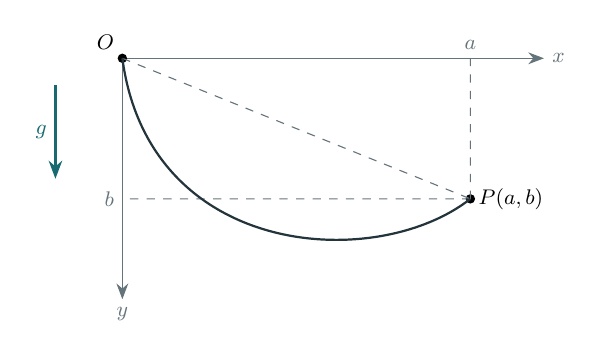
\begin{tikzpicture}[scale=.85,transform shape]

\draw[axis] (0,0)--(6.3,0) node[right] {$x$};
\draw[axis] (0,0)--(0,-3.6) node[below] {$y$};
\fill (0,0) circle (2pt) node[above left] {$O$};
\coordinate (P) at (5.2,-2.1);
\fill (P) circle (2pt) node[right] {$P(a,b)$};
\draw[guide] (P)--(5.2,0) node[above] {$a$};
\draw[guide] (P)--(0,-2.1) node[left] {$b$};
\draw[guide] (0,0)--(P);
\draw[object] (0,0) .. controls (.4,-3) and (3.8,-3.2) .. (P);
\draw[motion] (-1,-.4)--(-1,-1.8) node[midway,left] {$g$};

\end{tikzpicture}
\figcaption{图综二.3\quad 两端点和候选光滑轨道；坐标y沿重力方向向下。}
\end{minipage}\end{center}

\Needspace{6\baselineskip}\subsection*{解答}


图综二.3的$y$向下为正。能量守恒使任一高度处的速率只由$y$决定：
\[
v(y)=\sqrt{2gy}.
\]
较深处速度较大。终点离起点较远时，轨道先下降取得较大速度，再上升至指定终点。

把图A中的水平线看作薄层的交界面。相邻两层的折射率为$n_1,n_2$，光速为$c/n_1,c/n_2$，折射定律$n_1\sin\theta_1=n_2\sin\theta_2$便给出$\sin\theta/v$在界面两侧相同。也可直接把界面交点向右移$\delta x$。在交点左边，路长的一阶增量是$\sin\theta_1\,\delta x$，右边则减少$\sin\theta_2\,\delta x$。传播时间的一阶增量为$(\sin\theta_1/v_1-\sin\theta_2/v_2)\delta x$，驻值处括号为零。让各层变薄并取粒子的$v(y)$，得到
\[
\frac{\sin\theta}{v(y)}=\text{常量}.
\]
其中$\theta$是切线与竖直法线夹角。若切线与水平轴夹角为$\alpha$，则$\sin\theta=\cos\alpha$，连续极限下
\[
\frac{\cos\alpha}{\sqrt{2gy}}=\text{常量}.
\]
\begin{center}\begin{minipage}{.98\linewidth}\centering
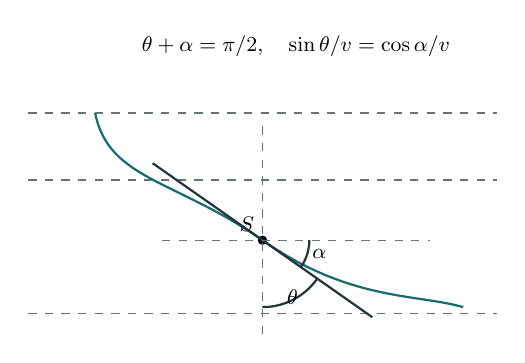
\begin{tikzpicture}[scale=.85,transform shape]

\foreach \y in {0,-1,-3}{\draw[guide] (-1,\y)--(6,\y);}
\draw[traj] (0,0) .. controls (.2,-1) and (1.2,-.99) .. (2.5,-1.9)
.. controls (3.8,-2.81) and (4.8,-2.7) .. (5.5,-2.9);
\coordinate (S) at (2.5,-1.9); \fill (S) circle (2pt) node[above left] {$S$};
\draw[object] (.86,-.75)--(4.14,-3.05);
\draw[guide] (2.5,-.2)--(2.5,-3.3);
\draw[guide] (1,-1.9)--(5,-1.9);
\draw[object] (3.2,-1.9) arc[start angle=0,end angle=-35,radius=.7];
\draw[object] (2.5,-2.9) arc[start angle=-90,end angle=-35,radius=1];
\node at (3.35,-2.1) {$\alpha$};
\node at (2.95,-2.75) {$\theta$};
\node at (3,1) {$\theta+\alpha=\pi/2,\quad \sin\theta/v=\cos\alpha/v$};

\end{tikzpicture}
\figcaption{解图综二.3A\quad 水平层的法线竖直，折射角与切线倾角互余。}
\end{minipage}\end{center}
解图综二.3A把入射角与切线倾角标在同一点。沿$x$增加的曲线有$\cos\alpha=1/\sqrt{1+y'^2}$，因而
\[
\boxed{y(1+y'^2)=A},\qquad A>0.
\]
时间泛函的被积式是$L=\sqrt{1+y'^2}/\sqrt{2gy}$，其中$y'=dy/dx$。$L$不显含$x$，沿驻值轨道的$L-y' L_{y'}$为常量。代入得$1/[\sqrt{2gy}\sqrt{1+y'^2}]$，正是图A由切线方向得到的同一常量。

为同时保留下降和上升的分支，令
\[
y=\frac A2(1-\cos\varphi),\qquad 0<\varphi<2\pi.
\]
此时
\[
y'^2=\frac Ay-1=\cot^2\frac\varphi2.
\]
沿一个无回绕摆线拱取$y'=\cot(\varphi/2)$，它在$\varphi=\pi$前为正、之后为负，与图B中下降段和上升段的方向相合。结合
$dy/d\varphi=(A/2)\sin\varphi$，得到
\[
\frac{dx}{d\varphi}
=\frac{(A/2)\sin\varphi}{\cot(\varphi/2)}
=\frac A2(1-\cos\varphi).
\]
在$\varphi=\pi$处，前式的商按化简后的连续值$A$取值。设$\beta=\varphi/2$，上式也就是$dx=2A\sin^2\beta\,d\beta$。起点对应$\beta=0$，积分为$x=\int_0^\beta A(1-\cos2u)\,du=A\beta-(A/2)\sin2\beta$。记$\mathcal R=A/2$，
\[
\boxed{x=\mathcal R(\varphi-\sin\varphi),\qquad
y=\mathcal R(1-\cos\varphi)}.
\]
它是摆线的第一个拱，起点处切线竖直，虽然初速为零，起步所需时间仍有限。
\begin{center}\begin{minipage}{.98\linewidth}\centering
\begin{tikzpicture}[scale=.85,transform shape]

\draw[axis] (0,0)--(6.8,0) node[right] {$x$};
\draw[axis] (0,0)--(0,-3) node[below] {$y$};
\draw[traj,domain=0:250,samples=220] plot ({.9*(rad(\x)-sin(\x))},{-.9*(1-cos(\x))});
\draw[guide,domain=250:330,samples=80] plot ({.9*(rad(\x)-sin(\x))},{-.9*(1-cos(\x))});
\fill (0,0) circle (2pt) node[above left] {$O$};
\fill (2.827433,-1.8) circle (2pt) node[below] {最低点$\varphi=\pi$};
\fill ({.9*(rad(250)-sin(250))},{-.9*(1-cos(250))}) circle (2pt) node[above right] {$P$示例};
\draw[motion] (0.968517,-1.266063)--(1.555586,-1.647310);
\draw[motion] (4.116674,-1.558218)--(4.767967,-1.301667);
\node at (3.3,1) {$x=\mathcal R(\varphi-\sin\varphi),\quad y=\mathcal R(1-\cos\varphi)$};
\node at (3.3,-4) {$a/b>\pi/2$时先降后升，末点在最低点之后};

\end{tikzpicture}
\figcaption{解图综二.3B\quad 单拱摆线在最低点前下降，过最低点后上升。}
\end{minipage}\end{center}
解图综二.3B标出$\varphi=\pi$的最低点和$\varphi>\pi$的上升段。终点条件为
\[
a=\mathcal R(\varphi_P-\sin\varphi_P),\qquad
b=\mathcal R(1-\cos\varphi_P).
\]
因此先解
\[
\boxed{\frac ab=
\frac{\varphi_P-\sin\varphi_P}{1-\cos\varphi_P}},
\quad 0<\varphi_P<2\pi,
\qquad
\boxed{\mathcal R=\frac b{1-\cos\varphi_P}}.
\]
这个比值从零严格增到无穷，故对任意$a,b>0$有唯一单拱解。例如求导分子可化为
$2(1-\cos\varphi)-\varphi\sin\varphi$；在$(0,\pi)$令$z=\varphi/2$，它为
$4\sin z(\sin z-z\cos z)>0$，在$(\pi,2\pi)$则两项都非负。
特别地
\[
\varphi_P\begin{cases}
<\pi,&a/b<\pi/2,\\
=\pi,&a/b=\pi/2,\\
>\pi,&a/b>\pi/2.
\end{cases}
\]
所以终点在最低点之前还是之后，应由横纵距离之比决定。

摆线弧长元与速率分别为
\[
ds=2\mathcal R\sin\frac\varphi2\,d\varphi,\qquad
v=2\sqrt{g\mathcal R}\sin\frac\varphi2,
\]
在$0<\varphi<2\pi$内正弦为正，因此
\[
dt=\sqrt{\frac{\mathcal R}{g}}\,d\varphi,
\qquad
\boxed{T_{\min}=\varphi_P\sqrt{\frac{\mathcal R}{g}}}.
\]
两个同时趋零的因子在起点相消，积分没有发散。
\begin{center}\begin{minipage}{.98\linewidth}\centering
\begin{tikzpicture}[scale=.85,transform shape]

\draw[axis] (0,0)--(8,0) node[right] {$x$};
\draw[axis] (0,0)--(0,-3.5) node[below] {$y$};
\foreach \a in {.45,.7,1,1.4}{
\draw[traj,domain=0:230,samples=170] plot ({\a*(rad(\x)-sin(\x))},{-\a*(1-cos(\x))});
}
\draw[force] (.7605,-1.17365)--(1.5265,-1.81665);
\node[right,text=warm] at (5.3,-.5) {$\nabla\mathcal T$沿切线};
\node at (4.7,1) {$|\nabla\mathcal T|=1/\sqrt{2gy}$};
\node at (4,-4.3) {沿摆线切向取等，任意其他路径满足$d\mathcal T\leq dt$};

\end{tikzpicture}
\figcaption{解图综二.3C\quad 同起点摆线族定义到达时间函数，梯度给最短时间的下界证明。}
\end{minipage}\end{center}
满足折射条件说明轨道使时间取驻值，还需比较任意其他路径。为确认它是最小值，解图综二.3C取由这些单拱摆线构成的轨道族。对任一点$(x,y)$、$x,y>0$，用唯一的$\mathcal R,\varphi$定义到达时间函数
\[
\mathcal T(x,y)=\varphi\sqrt{\frac{\mathcal R}{g}}.
\]
对两个参数分别微分，得到
\[
\mathcal T_x=\frac1{2\sqrt{g\mathcal R}},\qquad
\mathcal T_y=\frac{\cot(\varphi/2)}{2\sqrt{g\mathcal R}},
\qquad
|\nabla\mathcal T|=\frac1{\sqrt{2gy}}.
\]
具体地，将前两项乘$dx,dy$相加，$d\mathcal R$系数是
$[\varphi-\sin\varphi+\cot(\varphi/2)(1-\cos\varphi)]/(2\sqrt{g\mathcal R})
=\varphi/(2\sqrt{g\mathcal R})$，
$d\varphi$系数是$\sqrt{\mathcal R/g}$，恰为$d\mathcal T$。

沿任意可行轨道，柯西不等式给
\[
d\mathcal T=\nabla\mathcal T\cdot d\boldsymbol r
\leq |\nabla\mathcal T|\,ds
=\frac{ds}{\sqrt{2gy}}=dt.
\]
从起点积分，$\mathcal T(O)=0$，故
\[
T_{\rm path}\geq\mathcal T(P)
=\varphi_P\sqrt{\mathcal R/g}.
\]
摆线切向与$\nabla\mathcal T$同向，处处取等，因而达到这个下界。对$x<0$取偶延拓$\mathcal T(|x|,y)$。在$x$趋于零且$y>0$固定时，$\varphi\to0$，$\mathcal R(1-\cos\varphi)=y$给出$\mathcal T\to\sqrt{2y/g}$，同时$\mathcal T_x\to0$、$\mathcal T_y\to1/\sqrt{2gy}$。两侧的梯度在竖直轴上接合，因此同一不等式适用于整个$y>0$区域。

由能量守恒，可达区域为$y\geq0$。对可能接触$y=0$的轨道，取其沿正$y$方向平移$\varepsilon>0$的曲线作比较。平移保持$ds$，且$1/\sqrt{2g(y+\varepsilon)}\leq1/\sqrt{2gy}$，因此原轨道的时间满足
\[
T_{\rm path}\geq\mathcal T(a,b+\varepsilon)-\mathcal T(0,\varepsilon).
\]
这里$\mathcal T(0,\varepsilon)=\sqrt{2\varepsilon/g}$。令$\varepsilon\to0^+$，便得到从$O$到$P$的同一下界。


\Needspace{13\baselineskip}

\pdfbookmark[2]{第 4 题 线性引力下的闭合轨道与等效力心}{q4}

\section*{第 4 题\quad 线性引力下的闭合轨道与等效力心}\label{q:4}


设两个质点之间的吸引力与距离一次方成正比，写为
$\boldsymbol F=-GMm\,\boldsymbol r$，其中$\boldsymbol r$从施力质点指向受力质点，$G>0$的量纲按这个假设确定。
\begin{enumerate}
\item 太阳质量$M$固定，忽略行星对太阳的反作用。仿照轨道形状、面积规律和周期规律，建立这种引力下的三条行星运动定律。讨论轨道所在平面、椭圆力心位置及退化情况。
\item 若施力者为固定在$\boldsymbol R_i$处的若干质量$M_i>0$的质点，求受力质点一般轨道，说明能否用一个等效力心统一描述。
\end{enumerate}
讨论轨道时排除受力物体与实体施力物体相撞的情形。


\begin{center}\begin{minipage}{.98\linewidth}\centering
\begin{tikzpicture}[scale=.8,transform shape]

\draw[axis] (-.5,0)--(4.4,0) node[right] {$x$};
\draw[axis] (0,-.5)--(0,3.3) node[above] {$y$};
\fill (0,0) circle (2pt) node[below left] {$M$};
\fill (2.5,1.5) circle (2pt) node[right] {$m$};
\draw[guide] (0,0)--(2.5,1.5) node[midway,above left] {$\boldsymbol r$};
\draw[force] (2.5,1.5)--(1.25,.75) node[midway,below right] {$\boldsymbol F$};
\draw[motion] (2.5,1.5)--(3,3) node[above] {$\boldsymbol v$};
\begin{scope}[xshift=7cm]
\fill (-1,0) circle (2pt) node[left] {$M_1$};
\fill (1.5,1.8) circle (3pt) node[above] {$M_2$};
\fill (1.3,-1) circle (2pt) node[below] {$M_3$};
\fill (3,.4) circle (2pt) node[right] {$m$};
\draw[guide] (-1,0)--(3,.4); \draw[guide] (1.5,1.8)--(3,.4); \draw[guide] (1.3,-1)--(3,.4);
\end{scope}

\end{tikzpicture}
\figcaption{图综二.4\quad 单个线性中心力与任意固定源组，两种情形分别求轨道。}
\end{minipage}\end{center}

\Needspace{6\baselineskip}\subsection*{解答}


题设的力大小为$GMmr$，其中$G$的单位由力式确定为$\mathrm{kg^{-1}s^{-2}}$。将力的大小乘以朝向太阳的单位矢量，距离$r$便和单位矢量的分母约去，留下$-GMm\boldsymbol r$。这一步决定了分运动的形式。若$\boldsymbol r$与$x$轴夹角为$\theta$，则$F_x=-GMmr\cos\theta=-GMmx$、$F_y=-GMmr\sin\theta=-GMmy$。两个方向各有一条线性恢复力，弹性系数都为$GMm$，所以它们共有一个角频率。

图综二.4中力始终指向太阳。运动方程为
\[
\ddot{\boldsymbol r}=-GM\,\boldsymbol r=-\omega^2\boldsymbol r,
\qquad \omega=\sqrt{GM}.
\]
给定初位置$\boldsymbol r_0$和初速度$\boldsymbol v_0$，矢量解为
\[
\boxed{\boldsymbol r(t)=\boldsymbol r_0\cos\omega t+
\frac{\boldsymbol v_0}{\omega}\sin\omega t}.
\]
两个初矢量线性独立时，任意时刻的位置都在它们张成的平面内。只有一个独立方向时，运动退化为沿这条直线往复。两初矢量均为零时，质点静止在太阳所在的力心。
取$Oxy$为$\boldsymbol r_0,\boldsymbol v_0$张成的平面，则初始$z=\dot z=0$，且$\ddot z=-GMz$。这个一维初值问题的解恒为零，说明从平面内出发就留在平面内。对一般有心力，$\boldsymbol r\times\boldsymbol F=0$给固定的角动量方向，非零角动量同样确定运动平面。初始矢量共线时，沿该直线取一条坐标轴，其余两个坐标的初值与速度均为零，于是只剩轴上的振动。

\begin{center}\begin{minipage}{.98\linewidth}\centering
\begin{tikzpicture}[scale=.85,transform shape]

\draw[object] (0,0) ellipse (3 and 1.5);
\fill (0,0) circle (2pt) node[below left] {$O$太阳};
\draw[guide] (0,0)--(3,0) node[midway,below] {$\boldsymbol r_0$};
\draw[motion] (3,0)--(3,2) node[above] {$\boldsymbol v_0$};
\draw[force] (3,0)--(1.7,0) node[midway,above] {$\boldsymbol F$};
\node at (0,2.6) {图示为两初矢量正交的主轴坐标};
\node at (0,-2.7) {$\boldsymbol r(t)=\boldsymbol r_0\cos\omega t+
(\boldsymbol v_0/\omega)\sin\omega t$};

\end{tikzpicture}
\figcaption{解图综二.4A\quad 同频振动合成中心椭圆，力心在椭圆中心。}
\end{minipage}\end{center}
解图综二.4A把两个初矢量作为构造椭圆的两个系数。在平面直角坐标下，也可写为
\[
x=A\cos(\omega t+\phi_1),\qquad
y=B\cos(\omega t+\phi_2).
\]
振幅和相位可从初值直接读出。例如$x(0)=A\cos\phi_1$、$\dot x(0)=-A\omega\sin\phi_1$，所以$A^2=x(0)^2+[\dot x(0)/\omega]^2$，两式分别确定相位的余弦和正弦。$y$方向同理。令$u=\omega t+\phi_1$、$\delta=\phi_2-\phi_1$，则$x/A=\cos u$、$y/B=\cos u\cos\delta-\sin u\sin\delta$。把后一式移项后平方，再用$\sin^2u=1-\cos^2u$，就得到轨道方程。若某一振幅为零，轨道已在另一条轴上。

取两个振幅均为正的情形，消去$t$得到
\[
\boxed{\frac{x^2}{A^2}+\frac{y^2}{B^2}
-\frac{2xy}{AB}\cos(\phi_2-\phi_1)
=\sin^2(\phi_2-\phi_1)}.
\]
这个椭圆还可从初值直接求出长、短半轴。取一个以太阳为原点的平面直角坐标，把$\boldsymbol r_0$和$\boldsymbol v_0/\omega$作为两列组成矩阵$K$。若这两列不共线，则$x,y$的二次式写为$\boldsymbol r^{\mathsf T}(KK^{\mathsf T})^{-1}\boldsymbol r=1$。$KK^{\mathsf T}$的两个正特征值就是$a^2,b^2$，对应的单位特征矢量给主轴方向。这些值的和、积分别是
\[
a^2+b^2=|\boldsymbol r_0|^2+|\boldsymbol v_0|^2/\omega^2,\qquad
a^2b^2=|\boldsymbol r_0\times\boldsymbol v_0|^2/\omega^2.
\]
前一式说明能量决定两个半轴平方的和，后一式说明角动量决定椭圆的面积。给定初位置和初速度即可分别算出两半轴。若两个特征值相等，力心到轨道各点的距离相同，椭圆化为圆。若其中一个为零，线性变换把单位圆压在一条直线上，往、返两程各走同一个线段。

当$\phi_2-\phi_1$不是$\pi$的整数倍时，这是中心位于太阳的椭圆；旋转坐标可化为无交叉项的长短轴形式，圆为特殊情形。若相位差为$\pi$的整数倍，椭圆退化为直线段。点力模型中的质点沿直线穿过中心。有有限半径的太阳占据中心附近空间，此直线轨迹会碰到太阳。

由此第一条规律为：\textbf{非退化行星轨道为椭圆，太阳在各椭圆共同中心。}


中心力力矩为零：
\[
\frac d{dt}\left(m\boldsymbol r\times\dot{\boldsymbol r}\right)
=\boldsymbol r\times\boldsymbol F=0.
\]
第二条规律仍为：\textbf{太阳到行星的连线在相等时间扫过相等面积。}
面积速度是
\[
\dot{\mathcal A}
=\frac12|\boldsymbol r\times\dot{\boldsymbol r}|
=\frac{|\boldsymbol L|}{2m}.
\]
对主轴为$a,b$的参数解$x=a\cos\omega t,y=b\sin\omega t$，它还等于$ab\omega/2$，一周面积$\pi ab$。椭圆的极角速度由$\dot\theta=L_z/(mr^2)$给出。短轴端离太阳近，单位时间转过的极角大，长轴端则较小。振动相位的变化率$\omega$恒定，极角的变化率随矢径长度改变。

非共线时两个初矢量线性独立。图A的参数关系可看作将单位圆坐标$(\cos\omega t,\sin\omega t)$沿两个初矢量作线性变换，得到有面积的椭圆。半周期后位置变为$-\boldsymbol r$，正好走到椭圆的另一端。回到同一位置要求两个系数都回到初值，故最短公转周期等于两个分运动的共同周期。逐一对应开普勒三定律时，第一条改变了太阳在椭圆中的位置，第二条由中心力性质保留，第三条由角频率仅含$GM$得出同一太阳下的周期相等。

两个分运动频率相同，非退化轨道的最小公转周期是
\[
\boxed{T=\frac{2\pi}{\sqrt{GM}}}.
\]
所以第三条规律为：\textbf{围绕同一固定太阳的所有行星周期相同，与椭圆的大小、长短轴比以及行星质量无关。}

\begin{center}\begin{minipage}{.98\linewidth}\centering
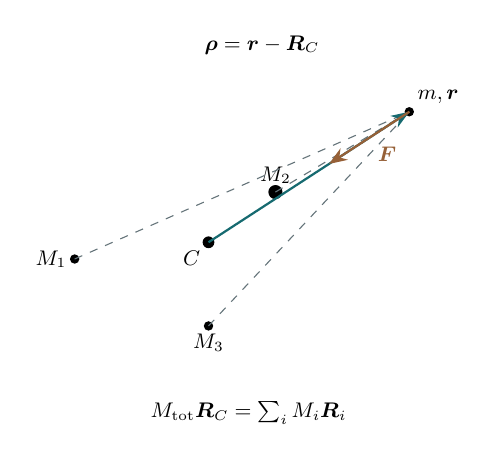
\begin{tikzpicture}[scale=.85,transform shape]

\fill (-1,0) circle (2pt) node[left] {$M_1$};
\fill (2,1) circle (3pt) node[above] {$M_2$};
\fill (1,-1) circle (2pt) node[below] {$M_3$};
\coordinate (C) at (1,.25); \fill (C) circle (2.5pt) node[below left] {$C$};
\coordinate (P) at (4,2.2); \fill (P) circle (2pt) node[above right] {$m,\boldsymbol r$};
\draw[guide] (-1,0)--(P); \draw[guide] (2,1)--(P); \draw[guide] (1,-1)--(P);
\draw[motion] (C)--(P);
\node at (1.8,3.2) {$\boldsymbol\rho=\boldsymbol r-\boldsymbol R_C$};
\draw[force] (P)--(2.8,1.42) node[midway,below right] {$\boldsymbol F$};
\node at (1.6,-2.3) {$M_{\rm tot}\boldsymbol R_C=\sum_iM_i\boldsymbol R_i$};

\end{tikzpicture}
\figcaption{解图综二.4B\quad 线性位置项求和后等效于总质量集中在固定质心。}
\end{minipage}\end{center}
第（2）问，解图综二.4B以任意固定原点表示源组位置。对受力点$\boldsymbol r$，
\[
\begin{aligned}
\boldsymbol F
&=-Gm\sum_iM_i(\boldsymbol r-\boldsymbol R_i)\\
&=-Gm\left[\left(\sum_iM_i\right)\boldsymbol r
-\sum_iM_i\boldsymbol R_i\right].
\end{aligned}
\]
定义源组总质量和质心
\[
M_{\rm tot}=\sum_iM_i,\qquad
\boldsymbol R_C=\frac{\sum_iM_i\boldsymbol R_i}{M_{\rm tot}},
\]
则
\[
\boxed{\boldsymbol F=-GmM_{\rm tot}(\boldsymbol r-\boldsymbol R_C)}.
\]
这个合力式在任意受力点成立，图B的三个源可以有任意空间分布。以$\boldsymbol \rho=\boldsymbol r-\boldsymbol R_C$为相对位置，
\[
\ddot{\boldsymbol \rho}+GM_{\rm tot}\boldsymbol\rho=0.
\]
把图B各虚线的方向统一为从$M_i$指向受力点。因作用力与这根矢量成正比，各项的受力点坐标都是同一个$\boldsymbol r$，可提出求和号。图示取$M_2=2M_1=2M_3$，所以$C$向$M_2$一侧偏移。把坐标原点移至$C$，新的初位置用$\boldsymbol r_0-\boldsymbol R_C$，初速度照旧。只要轨道与各固定质点在空间上分开，图A关于中心、面积和周期的结论便可逐一用于这组力。初相对位置与初速度共线且至少一个非零时，质点沿这条线往复。若初相对位置与速度都为零，它静止在$C$。

因此一般为以固定质心$C$为中心的平面椭圆，周期
$2\pi/\sqrt{GM_{\rm tot}}$；初相对位置与初速度共线时仍退化为直线段。
\begin{center}\begin{minipage}{.98\linewidth}\centering
\begin{tikzpicture}[scale=.8,transform shape]

\draw[guide] (0,0) circle (1); \draw[guide] (0,0) circle (2);
\draw[object] (0,0) ellipse (2.5 and 1.2);
\fill (0,0) circle (2pt) node[below left] {$C$};
\node at (0,3) {相对质心的等势圆与轨道};
\begin{scope}[xshift=6cm]
\draw[axis] (-2.3,0)--(2.3,0) node[right] {$s$};
\draw[axis] (0,-.3)--(0,3) node[above] {$U-U_0$};
\draw[traj,domain=-2:2,samples=100] plot (\x,{.6*\x*\x});
\node at (0,-1.4) {$U-U_0=GmM_{\rm tot}s^2/2$};
\end{scope}

\end{tikzpicture}
\figcaption{解图综二.4C\quad 源组位置只给势能增添常量，受力点的势能仍为各向同性二次型。}
\end{minipage}\end{center}
解图综二.4C用势能的负梯度$\boldsymbol F=-\nabla U$表示上述合力。
\[
\begin{aligned}
U&=\frac{Gm}{2}\sum_iM_i|\boldsymbol r-\boldsymbol R_i|^2\\
&=\frac{GmM_{\rm tot}}2|\boldsymbol r-\boldsymbol R_C|^2
+\frac{Gm}{2}\sum_iM_i|\boldsymbol R_i-\boldsymbol R_C|^2 .
\end{aligned}
\]
第二项不随受力点改变，只是势能零点的常量；第一项给出同一线性中心力。沿经过$C$的一条直径取有符号坐标$s$，图C的右半幅画的是这条直径上关于$s$的抛物线。
这种集中到质心的规律对源的位置没有对称性要求。通常的平方反比引力和库仑力则给每根位移矢量乘上各自距离的负三次方，系数随受力点移动而变化。球对称分布在球外可集中到球心，因为球对称使场在每个同心球面上等强，再由通量求出径向场。对于任意离散源组，各距离的权重需逐项保留。

解图综二.4D用最简单的两个等质量源说明，若要求任意源组都能集中到质心，力的径向大小为什么与距离成正比。设距离为$\ell$时的力写成$-GmM c(\ell)\boldsymbol\ell$。两个源各在$C$的左右$d$处，受力点$P$在垂直平分线上，离$C$为$s>0$。图D的两个水平分量互相抵消，竖直合力为$-2GmM s c(\sqrt{s^2+d^2})$。若等效为质心处总质量$2M$，竖直合力应为$-2GmM s c(s)$。比较得
\[
c(\sqrt{s^2+d^2})=c(s)\qquad(s>0,\ d>0).
\]
改变$d$可让左边的自变量取大于$s$的任意距离，故$c$在正半轴上为常量。线性力正满足这一关系，因而任意固定源组都可如此合并。
\begin{center}\begin{minipage}{.98\linewidth}\centering
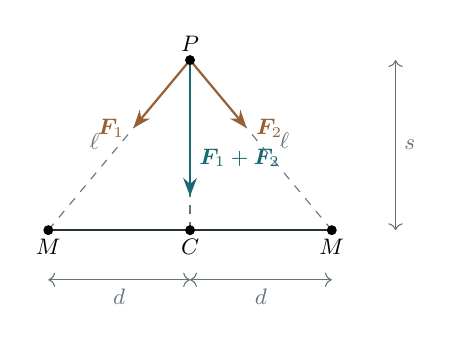
\begin{tikzpicture}[scale=.9,transform shape]
\coordinate (L) at (-2,0); \coordinate (C) at (0,0); \coordinate (R) at (2,0); \coordinate (P) at (0,2.4);
\draw[guide] (L)--(P) node[pos=.42,above left] {$\ell$};
\draw[guide] (R)--(P) node[pos=.43,above right] {$\ell$};
\draw[object] (L)--(R);
\draw[guide] (C)--(P);
\draw[force] (P)--(-.8,1.44) node[left] {$\boldsymbol F_1$};
\draw[force] (P)--(.8,1.44) node[right] {$\boldsymbol F_2$};
\draw[motion] (P)--(0,.48) node[pos=.72,right] {$\boldsymbol F_1+\boldsymbol F_2$};
\draw[axis,<->] (2.9,0)--(2.9,2.4) node[midway,right] {$s$};
\fill (L) circle (2pt) node[below] {$M$}; \fill (R) circle (2pt) node[below] {$M$};
\fill (C) circle (2pt) node[below] {$C$}; \fill (P) circle (2pt) node[above] {$P$};
\draw[axis,<->] (-2,-.7)--(0,-.7) node[midway,below] {$d$};
\draw[axis,<->] (0,-.7)--(2,-.7) node[midway,below] {$d$};
\end{tikzpicture}
\figcaption{解图综二.4D\quad 两个等质量源的合力沿垂直平分线。}
\end{minipage}\end{center}



\Needspace{13\baselineskip}

\pdfbookmark[2]{第 5 题 采样、空气质量与带电环的三个估算}{q5}

\section*{第 5 题\quad 采样、空气质量与带电环的三个估算}\label{q:5}


\begin{enumerate}
\item 一段电影中的轿车向前开，但轮胎上的三个完全相同图案看似不转。图案具有三重旋转对称性，相邻图案相隔$120^\circ$。以每秒24帧的等间隔采样模型，忽略曝光模糊，估计车轮纯滚动时出现这种现象的最低非零车速，并与学生百米短跑平均速度比较。车轮半径等参数应明确给出合理估值。
\item 移走教室内桌椅，只保留学生和教师，估计全体师生质量与室内空气质量之比。自行给出人数、空间与密度假设，说明结果的精度及参数依赖。
\item 半径$R$的细圆环均匀带有固定正电荷，总量$Q>0$。估算环所在平面内、距圆心$r\ll R$处的电场，给出方向及首项系数。可借轴上电场和小高斯柱，再从电势展开求近中心项。
\end{enumerate}


\begin{center}\begin{minipage}{.98\linewidth}\centering
\begin{tikzpicture}[scale=.8,transform shape]

\draw[object] (0,0) circle (1);
\draw[object] (0,0) circle (0.68);
\foreach \ang in {0,120,240}{
\begin{scope}[rotate=\ang]
\draw[object] (0.68,0) .. controls (0.83,0.19) and (0.93,0.16) .. (1,0);
\end{scope}
}

\node at (0,1.7) {三重图案};
\node at (0,-1.7) {24帧/秒};
\begin{scope}[xshift=4cm]
\draw[object] (-1.5,-1) rectangle (1.5,1);
\foreach \x in {-1,0,1}{\draw[object] (\x,.3) circle (.12);\draw[object] (\x,.18)--(\x,-.5);}
\node at (0,1.7) {师生与空气};
\node at (0,-1.7) {自行给参数估算};
\end{scope}
\begin{scope}[xshift=8.2cm]
\draw[object] (0,0) circle (1.1);
\fill (0,0) circle (1.5pt) node[below] {$O$};
\fill (.35,0) circle (2pt) node[right] {$P$};
\draw[guide] (0,0)--(60:1.1) node[midway,above left] {$R$};
\node at (0,1.7) {均匀带电环};
\node at (0,-1.7) {$OP=r\ll R$};
\end{scope}

\end{tikzpicture}
\figcaption{图综二.5\quad 三幅小图分别标出采样图案、空气空间与近中心观察点。}
\end{minipage}\end{center}

\Needspace{6\baselineskip}\subsection*{解答}


图综二.5的三个小图分别表示采样相位、人数与空气空间，以及环内近中心区域。前两问由给定物理关系估数量级，第三问用小量展开求首项系数。

24帧每秒意味着相机每隔$1/24\,\mathrm s$记录一次轮胎朝向。放映时看到的是这些离散的朝向，图A中间隔的转动由三重对称图案遮住了。给一个图案作记号，第一帧的记号在第二帧移动到相邻图案的初始位置，第三帧再移动到下一个初始位置。由于三个图案相同，这三幅图对不带记号的观察者一样。每帧转过一个重复角是最低非零情形，转过两个、三个重复角也会出现同一外观。

第（1）问，轮胎每转过$2\pi/3$外观重复一次。相邻帧时间$\Delta t=1/24\,\mathrm s$，若
\[
\omega\Delta t=n\frac{2\pi}{3},\qquad n=1,2,\ldots,
\]
各帧中图案的朝向相同。最小非零角速度为
\[
\boxed{\omega_{\min}=\frac{2\pi/3}{1/24}=16\pi\,\mathrm{s^{-1}}}.
\]
\begin{center}\begin{minipage}{.98\linewidth}\centering
\begin{tikzpicture}[scale=.85,transform shape]

\node at (0,1.7) {$t=0$};

\draw[object] (0,0) circle (0.85);
\draw[object] (0,0) circle (0.5780000000000001);
\foreach \ang in {0,120,240}{
\begin{scope}[rotate=\ang]
\draw[object] (0.5780000000000001,0) .. controls (0.7054999999999999,0.1615) and (0.7905,0.136) .. (0.85,0);
\end{scope}
}

\begin{scope}[xshift=3.3cm,rotate=120]

\draw[object] (0,0) circle (0.85);
\draw[object] (0,0) circle (0.5780000000000001);
\foreach \ang in {0,120,240}{
\begin{scope}[rotate=\ang]
\draw[object] (0.5780000000000001,0) .. controls (0.7054999999999999,0.1615) and (0.7905,0.136) .. (0.85,0);
\end{scope}
}

\end{scope}
\node at (3.3,1.7) {$t=1/24\,\mathrm s$};
\begin{scope}[xshift=6.6cm,rotate=240]

\draw[object] (0,0) circle (0.85);
\draw[object] (0,0) circle (0.5780000000000001);
\foreach \ang in {0,120,240}{
\begin{scope}[rotate=\ang]
\draw[object] (0.5780000000000001,0) .. controls (0.7054999999999999,0.1615) and (0.7905,0.136) .. (0.85,0);
\end{scope}
}

\end{scope}
\node at (6.6,1.7) {$t=2/24\,\mathrm s$};
\draw[motion] (1.1,0)--(2.2,0);
\draw[motion] (4.4,0)--(5.5,0);
\node at (3.3,-2) {每帧实转$2\pi/3$，图案外观相同};

\end{tikzpicture}
\figcaption{解图综二.5A\quad 三重图案在相邻采样帧中重复，产生静止假象。}
\end{minipage}\end{center}
解图综二.5A将相邻帧的相同图案对应起来。取小轿车轮胎半径$R_{\rm w}\simeq0.25\,\mathrm m$，纯滚动给
\[
v_{\min}=R_{\rm w}\omega_{\min}
\simeq12.6\,\mathrm{m/s}\simeq45\,\mathrm{km/h}.
\]
这相当于百米约8秒。若以学生百米12至17秒作比较，平均速度约6至8米每秒，所估轿车速度更高。半径减小时，最低混叠速度按$R_{\rm w}$减小。给定学生平均速度$u$，两者相等的半径是$u/(16\pi)$。换帧率或图案数时也可用同一采样关系重新比较。

第（2）问，先按人体体积作几何估算。设含教师共16人，平均单人体积$V_{\rm h}$。若教室高度约人体高度的2倍、宽度约人体宽度10倍、长度约人体厚度45倍，则教室体积约
\[
V_{\rm room}\sim2\times10\times45\,V_{\rm h}
=900V_{\rm h}.
\]
图B中人占据的部分与其余可供空气占据的空间要分开。用人体高度、宽度和厚度的乘积估计平均体积时，教室的三个倍数可以分别从层高、座椅竖列和前后排数估计。把讲台和走道的长度也折算进前后方向，得到图中采用的教室体积。于是人体总体积约占$16/900\simeq0.018$。把教室体积直接当空气体积只带来约百分之二的误差，远小于三个尺寸倍数的粗略程度。

密度比也可以从分子数密度来估算。人体含大量水，平均密度接近水。水与空气的平均摩尔质量分别约为$18$和$30\,\mathrm{g/mol}$，在这一粗略估算中，若气相分子间距按液相的十倍计，同体积液相约有$10^3$倍的分子数。乘上两者每个分子的质量之比$18/30$，密度比为几百，取$5\times10^2$作数量级计算。人体只占很小体积分数，密度高仍能使总质量与空气质量处于相近数量级。

全体人体体积为$16V_{\rm h}$，空气占据剩余$884V_{\rm h}$。若按稀疏气体与凝聚人体物质的差异，粗取
$\rho_{\rm h}/\rho_{\rm air}\sim5\times10^2$，
\[
\frac{M_{\rm h}}{M_{\rm air}}
=\frac{\rho_{\rm h}}{\rho_{\rm air}}
\frac{16}{900-16}\sim9\sim10.
\]
\begin{center}\begin{minipage}{.98\linewidth}\centering
\begin{tikzpicture}[scale=.85,transform shape]

\fill[accent!7] (0,0) rectangle (8,4);
\draw[object] (0,0) rectangle (8,4);
\foreach \x in {.5,1.5,...,7.5}{
\foreach \y in {.9,2.6}{
\fill[ink] (\x,{\y+.25}) circle (.11);
\draw[object] (\x,{\y+.14})--(\x,{\y-.3});
\draw[object] ({\x-.18},\y)--({\x+.18},\y);
}}
\node at (4,4.7) {16人占据一小部分室内空间};
\node at (4,-1) {$M_{\rm h}=N\bar m,\quad
M_{\rm air}=\rho_{\rm air}(V_{\rm room}-V_{\rm h,tot})$};

\end{tikzpicture}
\figcaption{解图综二.5B\quad 空气体积需扣除人体体积，再用各自密度换算质量。}
\end{minipage}\end{center}
再用图B的质量式代一组具体尺寸。16人平均50公斤，室内空间$8\times6\times3.5\,\mathrm{m^3}$，人体密度取$10^3\,\mathrm{kg/m^3}$、空气密度取$1.2\,\mathrm{kg/m^3}$。则
\[
M_{\rm h}\simeq800\,\mathrm{kg},\quad
V_{\rm h,tot}\simeq0.8\,\mathrm{m^3},
\]
\[
M_{\rm air}\simeq1.2(168-0.8)\simeq201\,\mathrm{kg},
\qquad
\boxed{M_{\rm h}/M_{\rm air}\simeq4}.
\]
两组估值从几倍到十倍。用人体作长度单位时估得较小的房间和较大的人体体积分数，用具体尺寸时估得较宽敞的房间。两组估值都显示人的总质量可与室内空气处于相近数量级。给定实际人数、平均质量和室内尺寸，就能用图B的同一组质量式计算。

第（3）问，取圆环轴为$z$，径向向外为正。轴上场由周向对称性求得
\[
E_z(0,z)=\frac{Qz}{4\pi\epsilon_0(R^2+z^2)^{3/2}}
\simeq\frac{Qz}{4\pi\epsilon_0R^3}
\quad(|z|\ll R).
\]
\begin{center}\begin{minipage}{.98\linewidth}\centering
\begin{tikzpicture}[scale=.85,transform shape]

\draw[object] (0,0) ellipse (3 and 1);
\draw[axis] (0,-2.6)--(0,2.7) node[above] {$z$};
\draw[object] (-.7,-.5)--(-.7,.5); \draw[object] (.7,-.5)--(.7,.5);
\draw[object] (0,.5) ellipse (.7 and .18); \draw[guide] (0,-.5) ellipse (.7 and .18);
\draw[force] (.2,.6)--(.2,1.8) node[right] {$E_z(\ell)$};
\draw[force] (.2,-.6)--(.2,-1.8) node[right] {$E_z(-\ell)$};
\draw[motion] (1.6,0)--(.7,0);
\draw[motion] (-1.6,0)--(-.7,0);
\node[right] at (1.6,.2) {$E_r$向内};
\draw[axis,<->] (-1.9,-.5)--(-1.9,.5) node[midway,left] {$2\ell$};
\node[below left] at (-.7,-.5) {$r$};
\node[above right] at (2.1,.75) {$R,Q$};
\node at (0,-3.5) {柱内无电荷，两端通量流出，侧面通量流入};

\end{tikzpicture}
\figcaption{解图综二.5C\quad 小高斯柱的端面与侧面通量决定径向场首项。}
\end{minipage}\end{center}
轴上的计算可直接从一个环元看出。到$(0,z)$的距离都是$\sqrt{R^2+z^2}$，库仑场的轴向投影再乘$z/\sqrt{R^2+z^2}$。绕轴的径向投影相互抵消，把轴向量按电荷积分就只留下总电量$Q$。近中心的轴向场与$z$同号，图C在两个端面用方向相反的箭头表示这一点。

柱面中的场可在圆心附近作光滑展开。轴对称使$E_z$对横向位移的首个修正为二次，环面对称使$E_z$对$z$为奇函数，因此端面上主项是与$z=\pm\ell$成正比的常量。侧面法向沿径向，轴向场在此处没有通量。$E_r$的首阶只与$r$有关，随$z$的改变量由偶次项给出。这样端面和侧面用的是同一阶的展开。

解图综二.5C取轴线重合、半径$r$、半高$\ell$的小高斯柱，$r,\ell\ll R$，整个柱内没有电荷。上端的轴向场分量向上，下端的轴向场分量向下，所以两端的向外通量均为正。端面各处的轴向场在首阶可用轴上的值，
\[
\Phi_{\rm ends}\simeq
2\frac{Q\ell}{4\pi\epsilon_0R^3}\pi r^2.
\]
侧面取向外径向场$E_r$，首阶沿高度变化可忽略，
\[
\Phi_{\rm side}\simeq E_r(2\pi r)(2\ell).
\]
高斯定律要求总通量为零，故
\[
2\frac{Q\ell}{4\pi\epsilon_0R^3}\pi r^2
+E_r4\pi r\ell=0,
\qquad
\boxed{\boldsymbol E(r,0)\simeq
-\frac{Qr}{8\pi\epsilon_0R^3}\hat{\boldsymbol r}}.
\]
场指向圆心。端面场“沿轴向流出”，侧面场须“沿径向流入”；这个方向也能在计算前判定。线性近似的相对修正从$(r/R)^2$阶开始。
\begin{center}\begin{minipage}{.98\linewidth}\centering
\begin{tikzpicture}[scale=.8,transform shape]

\draw[object] (0,0) circle (2.5);
\fill (0,0) circle (1.5pt) node[below left] {$O$};
\fill (.65,0) circle (2pt) node[below right] {$P$};
\coordinate (A) at (1.25,2.165); \fill (A) circle (2.5pt) node[above right] {$dq$};
\draw[guide] (0,0)--(A) node[midway,above left] {$R$};
\draw[guide] (.65,0)--(A) node[midway,right] {$\ell$};
\node at (1.8,3.3) {$\ell=\sqrt{R^2+r^2-2Rr\cos\psi}$};
\draw[object] (0,0)--(.65,0) node[midway,below] {$r$};
\draw[object] (.8,0) arc[start angle=0,end angle=60,radius=.8];
\node at (.9,.45) {$\psi$};
\node at (2,-3.5) {先对电荷元求势，再沿径向求导};

\end{tikzpicture}
\figcaption{解图综二.5D\quad 环元到近中心点的距离给出势积分中的分母。}
\end{minipage}\end{center}
在图D沿圆周逐个累加电荷元的电势，可以把线性近似延伸到更高阶。令$\rho=r/R$、$k_e=1/(4\pi\epsilon_0)$，电势为
\[
V(r)=\frac{k_eQ}{2\pi R}
\int_0^{2\pi}\frac{d\psi}
{\sqrt{1-2\rho\cos\psi+\rho^2}}.
\]
二阶展开被积函数：
\[
1+\rho\cos\psi-\frac{\rho^2}{2}
+\frac32\rho^2\cos^2\psi+O(\rho^3).
\]
周向平均用$\langle\cos\psi\rangle=0$、$\langle\cos^2\psi\rangle=1/2$，得二阶系数$-1/2+3/4=1/4$。对称性消去奇次幂。四阶项的系数为$3/8-(15/4)\cos^2\psi+(35/8)\cos^4\psi$。用$\langle\cos^2\psi\rangle=1/2$和$\langle\cos^4\psi\rangle=3/8$取平均，得到$9/64$，于是
\[
V=\frac{k_eQ}{R}
\left(1+\frac{\rho^2}{4}+\frac{9\rho^4}{64}+O(\rho^6)\right),
\]
\[
\boxed{E_r=-\frac{dV}{dr}
=-\frac{k_eQ}{R^2}
\left(\frac{\rho}{2}+\frac{9\rho^3}{16}+O(\rho^5)\right)}.
\]
圆心处的场为零，首个可能出现的是奇次项。这里积分求得的线性系数为负，方向和大小均与小柱通量式相同。三次项给出线性近似误差的首个量级。

把同一势积分写成闭式时，定义模数
$k^2=4\rho/(1+\rho)^2$及
\[
K(k)=\int_0^{\pi/2}\frac{d\theta}{\sqrt{1-k^2\sin^2\theta}},
\qquad
E(k)=\int_0^{\pi/2}\sqrt{1-k^2\sin^2\theta}\,d\theta.
\]
从图D还可把同一个势积分化成椭圆积分。电荷元取$dq=Q\,d\psi/(2\pi)$，将距离平方中的$1-2\rho\cos\psi+\rho^2$写为$(1+\rho)^2[1-k^2\cos^2(\psi/2)]$。代入后把整周按半角对称性折到$0\le\theta\le\pi/2$，就得到下式中的$K(k)$。利用$dK/dk=E/[k(1-k^2)]-K/k$对势求导，再用$1-k^2=(R-r)^2/(R+r)^2$整理，得到同一个径向场。这里的精确式还可用于较大的$r/R$，它的低阶展开则说明哪些项必须同时保留。

在$0<r<R$内，径向分量写成下式。中心处取$r\to0^+$的极限，$E_r$趋于零。
\[
V=\frac{2k_eQ}{\pi(R+r)}K(k),\qquad
E_r=\frac{k_eQ}{\pi r}
\left[\frac{K(k)}{R+r}-\frac{E(k)}{R-r}\right].
\]
方括号的常数项和线性项相消，因而把$K,E$都展开到$k^4$，
\[
K=\frac\pi2\left(1+\frac{k^2}{4}+\frac{9k^4}{64}+\cdots\right),
\quad
E=\frac\pi2\left(1-\frac{k^2}{4}-\frac{3k^4}{64}+\cdots\right).
\]
用$k^2=4\rho-8\rho^2+\cdots$换回$\rho$，
\[
K=\frac\pi2(1+\rho+\rho^2/4+\cdots),\quad
E=\frac\pi2(1-\rho+5\rho^2/4+\cdots).
\]
沿过圆心的直径，电势为偶函数，电场分量为奇函数。因此，径向场式方括号中的量与$r E_r$成正比，只含偶次幂，可写成$-\pi\rho^2/(2R)+O(\rho^4/R)$。再次得到
$E_r=-k_eQr/(2R^3)+O(r^3)$。
为看清相消，先把$K,E$各除以$\pi/2$，再分别乘$R/(R+r)$与$R/(R-r)$。两项乘积都以1起头，线性项均为零，二次系数分别为$1/4$和$5/4$，相减才留下$-\rho^2$。外面的$1/r$把它变成电场的一次项。因为$k^2$本身与$\rho$同阶，$k^4$项恰好参与这个二次系数。保留这部分后，精确积分和小柱通量给出相同方向和系数。



\Needspace{13\baselineskip}

\pdfbookmark[2]{第 6 题 水平磁场中带电圆环由滑动到滚动}{q6}

\section*{第 6 题\quad 水平磁场中带电圆环由滑动到滚动}\label{q:6}


半径$R$、质量$m$的均匀细圆环竖立在绝缘水平地面上，固定在环上的均匀正电荷总量为$Q>0$。圆环位于东西方向的竖直平面，$t=0$时以$v_0\geq0$向东平动，初始角速度为零。均匀磁场沿水平向北，即垂直纸面向里，大小$B>0$；圆环与地面间滑动摩擦因数$\mu>0$，忽略形变、辐射及空气阻力。
\begin{enumerate}
\item 求圆环始终不离地的$v_0$范围，分别说明临界初速与零初速时的运动。
\item 在能够达到纯滚动的范围内，求此前的$v(t)$，并写出转速、支持力与滑动结束的条件。
\item 若$v_0=mg/(2QB)$，求首次纯滚动时刻$T$，并说明之后的运动。
\end{enumerate}
从各带电弧元的洛伦兹力出发，求磁合力和绕环心的总力矩。


\begin{center}\begin{minipage}{.98\linewidth}\centering
\begin{tikzpicture}[scale=.8,transform shape]

\draw[object] (0,0) circle (2);
\draw[object] (-3,-2)--(3.5,-2);
\draw[guide] (0,0)--(-45:2) node[midway,above right] {$R$};
\node at (0,2.7) {$m,Q$};
\draw[motion] (2.4,0)--(4.2,0) node[right] {$v_0$向东};
\foreach \x in {-2.8,2.8}{
\draw[object] (\x,1.8) circle (.12);
\draw[object] ({\x-.085},1.715)--({\x+.085},1.885);
\draw[object] ({\x-.085},1.885)--({\x+.085},1.715);
}
\node[left] at (-2.95,1.8) {$B$向北};
\node[below] at (0,-2.2) {绝缘地面，$\mu$};

\end{tikzpicture}
\figcaption{图综二.6\quad 圆环最初仅平动，磁场垂直纸面向里。}
\end{minipage}\end{center}

\Needspace{6\baselineskip}\subsection*{解答}


图综二.6取东向为$x$正、竖直向上为$y$正、纸外为$z$正，故$\boldsymbol B=-B\hat{\boldsymbol z}$。顺时针角速度的大小记为$\omega\geq0$，角速度矢量为$-\omega\hat{\boldsymbol z}$。

从图上的一个电荷元出发，分别计算平动与转动两项磁力，再求整个圆周的积分。弧元位置相对环心为$\boldsymbol r$，其地面系速度为
$\boldsymbol v+\boldsymbol\omega\times\boldsymbol r$，受力
\[
d\boldsymbol F=dq\,\boldsymbol v\times\boldsymbol B
+dq\,(\boldsymbol\omega\times\boldsymbol r)\times\boldsymbol B.
\]
\begin{center}\begin{minipage}{.98\linewidth}\centering
\begin{tikzpicture}[scale=.78,transform shape]

\draw[guide] (0,0) circle (2);
\coordinate (P) at (1.414,1.414); \fill (P) circle (2pt) node[left] {$dq$};
\draw[guide] (0,0)--(P) node[midway,left] {$\boldsymbol r$};
\draw[motion] (P)--(3.6,1.414) node[right] {$\boldsymbol v$};
\draw[motion] (P)--(2.6,.228) node[right] {$\boldsymbol\omega\times\boldsymbol r$};
\draw[force] (P)--(1.414,3.3) node[above] {$dq\,\boldsymbol v\times\boldsymbol B$};
\draw[force] (P)--(2.7,2.7) node[above right] {转动项径向向外};
\node at (-1.4,2.6) {$\boldsymbol B=-B\hat{\boldsymbol z}$};
\node at (1,-3) {径向磁力的合力与力矩均为零；均匀平动项的总力矩也为零};

\end{tikzpicture}
\figcaption{解图综二.6A\quad 单弧元的速度分解与洛伦兹力分解。}
\end{minipage}\end{center}
洛伦兹力用弧元相对地面的速度计算。图A中环心的平动速度对各弧元都一样，因而这一部分磁力也同向。转动速度沿圆周切线，不同弧元的切向随位置转过同样的角度。对图中的任意弧元，$\boldsymbol r$在环平面内，有$\boldsymbol r\cdot\boldsymbol B=0$，而$\boldsymbol\omega\cdot\boldsymbol B=\omega B$。利用三重积恒等式，
\[
(\boldsymbol\omega\times\boldsymbol r)\times\boldsymbol B
=\boldsymbol r(\boldsymbol\omega\cdot\boldsymbol B)
-\boldsymbol\omega(\boldsymbol r\cdot\boldsymbol B)
=\omega B\boldsymbol r.
\]
所以图A的径向箭头对每个弧元都指向环外。相对的两段弧电荷相等，径向力方向相反。平动项的两个力方向相同，力臂方向相反，它们关于环心的力矩相消。

解图综二.6A中平动项对所有电荷元都沿向上方向，每份力与$dq$成正比；转动项沿径向向外，大小为$dq\,\omega BR$。均匀圆周上
$\int\boldsymbol r\,dq=0$，所以转动项的合力为零；该项各自沿半径，绕环心力矩也为零。

平动项的总力为$Q\boldsymbol v\times\boldsymbol B$，而其绕环心的总力矩
\[
\int\boldsymbol r\times(dq\,\boldsymbol v\times\boldsymbol B)
=\left(\int\boldsymbol r\,dq\right)\times
(\boldsymbol v\times\boldsymbol B)=0.
\]
故整体受向上的磁力$F_B=QBv$，没有磁力矩。对保持接地的圆环，
\[
\boxed{N=mg-QBv}.
\]
\begin{center}\begin{minipage}{.98\linewidth}\centering
\begin{tikzpicture}[scale=.85,transform shape]

\draw[object] (0,0) circle (2); \draw[object] (-3,-2)--(3.5,-2);
\draw[force] (0,0)--(0,1.5);
\node[right] at (.5,1) {$QBv$};
\draw[force] (0,0)--(0,-1) node[left] {$mg$};
\draw[force] (0,-2)--(0,-1.1) node[right] {$N$};
\draw[force] (0,-2)--(-2,-2) node[below] {$f=\mu N$};
\draw[motion] (0,0)--(3,0) node[right] {$v$};
\node at (0,2.8) {$N=mg-QBv\geq0$};
\node at (0,-3.3) {摩擦减速并给顺时针力矩；磁力绕心总矩为零};

\end{tikzpicture}
\figcaption{解图综二.6B\quad 整体竖直平衡、向西摩擦与向东平动。}
\end{minipage}\end{center}
图B的$N$表示地面对环的竖直支持力，大小等于环压地面的力。环心高度保持为$R$时，向上的$N$和$QBv$合起来平衡重力。最初接触点与环心都有同样的向东速度，摩擦因此向西。滑动时$\dot v\le0$，所以只要初始支持力为正，随着$v$减小，$N$会增大。恰在$v_0=v_c$时，重力与平动磁力相抵，初始高度和速度可保持。若$v_0>v_c$，重力小于向上的磁力，即使支持力为零仍有向上加速度，环随即升离地面。

解图综二.6B显示磁力减小支持力，摩擦则向西，既减慢平动又使环顺时针转。只要起初不离地，之后平动减速使磁力更小，因此
\[
\boxed{0\leq v_0\leq v_c,\qquad v_c=\frac{mg}{QB}}.
\]
$v_0=0$时圆环静止。$v_0=v_c$时$N=f=0$，圆环保持初始平动速度和零角速度。$0<v_0<v_c$时有向西摩擦及顺时针角加速度，圆环经过滑动进入纯滚动。

滑动阶段接触点向东相对地面运动，$f=\mu N$向西。平动方程
\[
m\dot v=-\mu(mg-QBv)
=\mu QB(v-v_c).
\]
方程中随时间变化的是$v$和$N$。在$0<v_0<v_c$的滑动阶段，$mg-QBv>0$。分离变量后的积分可用这一正量在初态和当前时刻的比值写成对数。用初速度和当时速度作积分端点，可写成
\[
\mu t=\int_{v_0}^{v(t)}\frac{m\,du}{QBu-mg}
=\frac{m}{QB}\ln\frac{mg-QBv(t)}{mg-QBv_0}.
\]
速度降低使对数的分子变大，与滑动时间为正相合。指数形式可用图C的曲线斜率理解。开始时斜率由最初的摩擦力给出，后来支持力增加，曲线向下变陡。

令$\tau=m/(\mu QB)$，分离变量并用$v(0)=v_0$：
\[
\frac{dv}{v-v_c}=\frac{dt}{\tau},
\quad
\boxed{v(t)=v_c-(v_c-v_0)e^{t/\tau}}\qquad(0\leq t\leq T).
\]
于是
\[
\boxed{N(t)=(mg-QBv_0)e^{t/\tau}}.
\]
支持力随平动减慢而增大，摩擦也增大。指数增大的量是$v_c-v$，它与支持力成正比。

图B中$N$的作用线经过环心，重力也作用在环心。磁力的两项绕环心都给零总力矩，故只剩地面摩擦的力矩$fR$。对时段$0$到$t$，把平动动量减量和转动角动量增量写成同一个摩擦冲量$J_f=\int_0^tf\,dt$，有$m(v_0-v)=J_f$、$I\omega=RJ_f$。在细环中$I=mR^2$，所以环缘的转动速度增量恰等于环心的平动速度减量。这也解释图C滑动段两条曲线的斜率大小相等、符号相反。

细环惯量$I=mR^2$，唯一非零绕心力矩来自摩擦：
\[
I\dot\omega=fR,\qquad
R\dot\omega=\frac fm=-\dot v.
\]
积分得
\[
\boxed{R\omega=v_0-v}.
\]
\begin{center}\begin{minipage}{.98\linewidth}\centering
\begin{tikzpicture}[scale=.85,transform shape]

\draw[axis] (0,0)--(6.8,0) node[right] {$t/\tau$};
\draw[axis] (0,0)--(0,4.3) node[above] {$v/v_c,\ R\omega/v_c$};
\draw[traj,domain=0:.405465,samples=120] plot ({10*\x},{7*(1-.5*exp(\x))});
\draw[force,domain=0:.405465,samples=120] plot ({10*\x},{7*(.5*exp(\x)-.5)});
\draw[object] (4.05465,1.75)--(6,1.75);
\draw[guide] (4.05465,0)--(4.05465,3.5);
\node[below] at (4.05465,0) {$\ln(3/2)$};
\node at (2.6,3.4) {$v/v_c$}; \node at (2.7,.5) {$R\omega/v_c$};
\node[right] at (6,1.75) {$1/4$};
\node at (3.3,5) {$v_0=v_c/2,\quad v-R\omega=2v-v_0$};
\node at (3.3,-1.5) {交点后平动速度与环缘转动速度保持相等};

\end{tikzpicture}
\figcaption{解图综二.6C\quad 平动减慢与自转加快在首次滚动时相接。}
\end{minipage}\end{center}
环底相对环心的转动速度向西，大小$R\omega$。地面看到的接触点速度为这两个速度的矢量和。图C以$v_c$为速度单位，两条曲线的纵坐标差乘$v_c$，便得到接触点向东的滑速。两条曲线首次相交时，接触点瞬时静止，平动和自转从同一纵坐标继续保持常量。在纯滚动阶段把接触力写成待求的静摩擦，再用滚动关系求得它为零。

解图综二.6C中接触点滑速为$v-R\omega=2v-v_0$；它第一次降为零时
\[
\boxed{v(T)=\frac{v_0}{2},\qquad
\omega(T)=\frac{v_0}{2R}}.
\]
把这个速度代入指数式，
\[
e^{T/\tau}=\frac{v_c-v_0/2}{v_c-v_0},
\quad
\boxed{T=\frac{m}{\mu QB}
\ln\frac{v_c-v_0/2}{v_c-v_0}}.
\]
$0<v_0<v_c$时分子、分母均为正，分子更大，故$T>0$。图C的指数段止于$v=v_0/2$，其后由纯滚动的受力方程决定。

第（3）问，$v_0=v_c/2$，于是
\[
\boxed{T=\frac{m}{\mu QB}\ln\frac32}.
\]
达到滚动后，水平受力和绕心力矩若仍有静摩擦$f_s$，则
$m\dot v=-f_s$、$mR^2\dot\omega=f_sR$，而滚动约束要求$\dot v=R\dot\omega$；三式只允许$f_s=0$。因此保持
\[
v=v_0/2,\qquad \omega=v_0/(2R),
\qquad N=mg-QBv_0/2>0.
\]
磁力对每个电荷元都不做功，整体的动能损失来自接触滑动：
\[
K_i=\frac12mv_0^2,\qquad
K_f=\frac12m\left(\frac{v_0}{2}\right)^2
+\frac12mR^2\left(\frac{v_0}{2R}\right)^2
=\frac14mv_0^2.
\]
故摩擦耗散为 $mv_0^2/4$。也可以直接用图C中的纵坐标差：滑动速度为 $v-R\omega=2v-v_0$，滑动摩擦力大小为 $f$，平动方程给 $f\,\mathrm dt=-m\,\mathrm dv$。每一小段产生的热量由摩擦冲量乘当时的滑速得到，累加为
\[
Q=\int_0^T f(2v-v_0)\,\mathrm dt
  =m\int_{v_0/2}^{v_0}(2v-v_0)\,\mathrm dv=\frac{mv_0^2}{4}.
\]
磁场通过支持力改变进入滚动的时长。薄环的终速 $v_0/2$ 由平动与转动的共同冲量关系确定，所以耗散也仅由这两个端点的速度决定。


\end{document}
